\chapter{System Modelling}
\label{system_modelling}

\emph{This chapter presents the mathematical description of hydraulic components in water distribution networks. Thereby, the physical measures of hydraulic systems are introduced. The similarities to electronic networks are shown by explaining the relevant properties of graph theory. The model of a single and multi-inlet network, based on \cite{oneinput_paper}, is first introduced, then the model description is extended such that it is capable of handling multiple Water Tanks. In the end of the chapter, different models are compared and a summary of the extended system model is given.}

\section{Hydraulic component modelling}
\label{hydraulic_component_modelling}

In this section the mathematical relation between pressure and flow is given for each component in a WSS system, in order to show the non-linear behaviour of the water flowing through them. Here the purpose is not to derive the different component models, but to introduce the mathematical formalism which describes them.

\eqref{onecomponent} shows the dual variable which describes all two-terminal components in a hydraulic network 

\begin{equation}
\label{onecomponent}
 \begin{pmatrix}
    \Delta p \\
    q
\end{pmatrix}
=
 \begin{pmatrix}
    p_{in} - p_{out} \\
    q
\end{pmatrix},
\end{equation}



 \begin{minipage}[t]{0.20\textwidth}
where\\
\hspace*{8mm} $\Delta p$ \\
\hspace*{8mm} $q$ \\
\hspace*{8mm} $p_{in}$, $p_{out}$ 
\end{minipage}
\begin{minipage}[t]{0.68\textwidth}
\vspace*{2mm}
is the differential pressure across the element,\\
is the flow through the element,\\
are the absolute pressures at the two endpoints.
\end{minipage}
\begin{minipage}[t]{0.10\textwidth}
\vspace*{2mm}
\textcolor{White}{te}$\unit{Pa}$\\
\textcolor{White}{te}$\unit{m^3/s}$\\
\textcolor{White}{te}$\unit{Pa}$
\end{minipage}

\subsection{Hydraulic head}
\label{hydraulic_head}

As can be seen in \eqref{onecomponent}, the measure of pressure is in $[Pa]$ and the measure of volumetric flow is in $[\frac{m^3}{s}]$. In the further report SI units are used, in order to show the hydraulic model of the components. However, non-SI units are also utilized due to the fact that EPANET uses meter head for pressure and liters per seconds for flow simulations. Furthermore, the measurements carried out on the Randers network are also measured in non-SI units. Therefore, we allow ourselves to use non-SI units for showing measurement and simulation results. 

The unit conversion between liters and cubic meters yields by a constant, while meter head expresses pressure in terms of length. The relation between pressure and pressure head is explained in \eqref{pressurehead}. 

%\begin{ceqn} 
\begin{equation}
\label{pressurehead}
  h_p = \frac{p}{\rho g}.
\end{equation} 
%\end{ceqn} 

\begin{minipage}[t]{0.20\textwidth}
where\\
\hspace*{8mm} $h_p$ \\
\hspace*{8mm} $p$ \\
\hspace*{8mm} $g$ \\
\hspace*{8mm} $\rho$ 
\end{minipage}
\begin{minipage}[t]{0.63\textwidth}
\vspace*{2mm}
is the pressure head,\\
is the absolute pressure in pascals, \\
is the gravitational constant, \\
is the density of the fluid.
\end{minipage}
\begin{minipage}[t]{0.15\textwidth}
\vspace*{2mm}
\textcolor{White}{te}$\unit{m}$\\
\textcolor{White}{te}$\unit{kg/ms^2}$\\
\textcolor{White}{te}$\unit{m/s^2}$\\
\textcolor{White}{te}$\unit{kg/m^3}$
\end{minipage}

As can be seen in \eqref{pressurehead}, if the density of the liquid is a known parameter, the conversion can be done easily between pressure and pressure head. In the thesis, the fluid is water and its density is assumed to be constant. 

In general, the hydraulic head and total head is a measure of the potential of fluid at a specific measurement point. It relates the energy of an incompressible fluid to the height of an equivalent static column of the fluid. The different forms of energies regarding fluids can be measured in distance, and therefore the reason is that these terms are referred to as heads. The total hydraulic head of a fluid is composed of the pressure head and elevation head. \footnote{There is a third term, called the kinetic head which is discarded, since the velocity of the fluid is assumed to be constant along the cross sectional area in the whole length of pipes \cite{chen2016sustainable}.} The total head is given in \eqref{totalhead}.

%\begin{ceqn} 
\begin{equation}
\label{totalhead}
  h_t = h_p + z,
\end{equation}
%\end{ceqn} 

\begin{minipage}[t]{0.20\textwidth}
where\\
\hspace*{8mm} $h_t$ \\
\hspace*{8mm} $z$ 
\end{minipage}
\begin{minipage}[t]{0.68\textwidth}
\vspace*{2mm}
is the total head,\\
is the elevation(head).
\end{minipage}
\begin{minipage}[t]{0.10\textwidth}
\vspace*{2mm}
\textcolor{White}{te}$\unit{m}$\\
\textcolor{White}{te}$\unit{m}$
\end{minipage}

Therefore, pressure head is a measurement of length which depends on the density of the fluid but can be converted to pressure units such as Pascals. Using meters for describing pressure in the system is convenient due to the reason that pressure can be treated the same way as elevation. During the derivation of the WSS network model this property is going to be strongly exploited. 

\subsection{Pipe model}
\label{pipe_component}

Pipes in the network are governed by the dynamics shown in \eqref{complete_pipemodel}.

\begin{equation}
\label{complete_pipemodel}
  \Delta p_i = J_i \dot{q_i} + f_i(q_i) - h_i,
\end{equation}

 \begin{minipage}[t]{0.20\textwidth}
where\\
\hspace*{8mm} $J_i$ \\
\hspace*{8mm} $f_i(q_i)$ \\
\hspace*{8mm} $ h_i$ 
\end{minipage}
\begin{minipage}[t]{0.68\textwidth}
\vspace*{2mm}
is the mass inertia of the water in the $i^{th}$ pipe,\\ 
is the pressure drop due to friction in the $i^{th}$ pipe,\\
is the pressure drop due to geodesic level difference across the two terminals of the $i^{th}$ pipe.
\end{minipage}

The dynamics due to mass inertia are discarded in the thesis, as it is shown in other works that the small time constant of these mass inertia dynamics are not dominant in the system if there are elevated reservoirs included \cite{8thsemester_project,kenneth_houe}. Therefore, the pressure drop across pipes can be written as

\begin{equation}
\label{complete_pipemodel1}
  \Delta p_i = f_i(q_i) - h_i.
\end{equation}

Additionally, the dynamics due to inertia of the liquid are not the only possible dynamics for pipes. The phenomenon, called water hammer occurs when a fluid, or gas in motion is forced to stop or change direction suddenly. This can occur when a valve is rapidly closed or opened. In this case, a pressure wave runs through the pipe, causing vibration and possible damage to the network \cite{2011water}. However, \eqref{complete_pipemodel} models the pressure drops or equivalently, the headloss, due to the elevation of the pipes and friction of the fluid. Although such a rapid change can occur in the network due to undesired network operation, in the further modelling normal operation is assumed.

The pressure drop due to friction across the $i^{th}$ pipe segment is a diagonal map where $f: \mathbb{R}^{m} \rightarrow \mathbb{R}^{m} $ is strictly increasing.\footnote{A map $f: \mathbb{R}^{m} \rightarrow \mathbb{R}^{m} $ is strictly increasing if $\langle x-y, f(x)-f(y) \rangle > 0$ for every $x,y \in \: \mathbb{R}^{m}$ such that $x \neq y$ \cite{oneinput_paper}.} As it is shown in \eqref{deltap_friction}, $f_i$ describes a flow dependant pressure drop due to the hydraulic resistance such that

\begin{equation}
  \label{deltap_friction}
  f_i(q_i) = \gamma_i |q_i|q_i,
\end{equation}

 \begin{minipage}[t]{0.20\textwidth}
where\\
\hspace*{8mm} $\gamma_i > 0$ 
\end{minipage}
\begin{minipage}[t]{0.68\textwidth}
\vspace*{2mm}
is the resistance coefficient, the parameter of pipes. 
\end{minipage}
\begin{minipage}[t]{0.10\textwidth}
\vspace*{2mm}
\textcolor{White}{te}$\unit{\cdot}$
\end{minipage}

\eqref{deltap_friction} is motivated by turbulent flow in the pipes, which is typical in water supply applications. Furthermore, the resistance coefficients are calculated according to the Darcy-Weisbach formula, which provides the theoretically most precise result and is the most commonly used friction calculation in Europe\cite{prahata,agency2016epanet}. $\gamma$ is given as shown in \eqref{resistance_coefficient} \footnote{ Among other calculation methods, it is possible to use D-W friction calculator in EPANET. }.  

\begin{equation}
  \label{resistance_coefficient}
  \gamma(q) = \frac{c_D f_{D}(\epsilon,Re(q), D )l}{D^{5}},
\end{equation}

 \begin{minipage}[t]{0.20\textwidth}
where\\
\hspace*{8mm} $f_{D}$ \\
\hspace*{8mm} $\epsilon$ \\
\hspace*{8mm} $D$ \\
\hspace*{8mm} $Re$ \\
\hspace*{8mm} $c_D$ \\
\hspace*{8mm} $l$ 
\end{minipage}
\begin{minipage}[t]{0.68\textwidth}
\vspace*{2mm}
is the Darcy friction factor,  \\
is the roughness of the pipe segment,  \\
is the diameter of the pipe segment,  \\
is the Reynolds-number,  \\
is the D-W  coefficient for SI units,  \\
is the length of the pipe segment.
\end{minipage}
\begin{minipage}[t]{0.10\textwidth}
\vspace*{2mm}
\textcolor{White}{te}$\unit{\cdot}$\\
\textcolor{White}{te}$\unit{m}$\\
\textcolor{White}{te}$\unit{m}$ \\
\textcolor{White}{te}$\unit{\cdot}$ \\
\textcolor{White}{te}$\unit{s^2/m}$ \\
\textcolor{White}{te}$\unit{m}$
\end{minipage}

In \eqref{resistance_coefficient}, the Darcy friction factor $f_D$ depends on the Reynolds number, which is determined by the volumetric flow in the pipes. At high flows Re becomes nearly constant and therefore normally this flow dependency is disregarded. Thus, $f_D$ is considered to be constant in the simulations based on this type of network modelling. 

Furthermore, it is important to note that $f_i(\cdot)$ is a homogeneous map which means that if the terms in its argument are multiplied by a positive scalar, then its value is multiplied by some power of this scalar \footnote{$g(\alpha v) = \alpha^k g(v)$}. For $f_i(q_i)$, it has been shown in \cite{oneinput_paper} that

\begin{equation}
  \label{homogeneity}
  \gamma_i |(\alpha q_i)|(\alpha q_i) = f_i(\alpha q_i) = \alpha^2 f_i(q_i).
\end{equation}

More precisely, with the given structure of $f(\cdot)$ the scaling would be $|\alpha|\alpha$, however $\alpha \geq 0$ is already assumed in \eqref{homogeneity}. 
This property is noted here and used later in the network modelling, in \secref{multi_inlet_reduced_network_description}, where the scaling is indeed such that $\alpha \in \: \mathbb{R}_{+}$. In the following, it is assumed that each $f_i$ for the $i^{th}$ pipe segment has a structure as shown in \eqref{deltap_friction}.

\subsection{Valve model}
\label{valve_component}

Valves in the network are governed by the algebraic expression shown in \eqref{valvemodel}.

\begin{equation}
\label{valvemodel}
 \Delta p_i = \mu_i(q_i,k_v) = \frac{1}{k_v(OD)^2} |q_i| q_i, 
\end{equation}

 \begin{minipage}[t]{0.20\textwidth}
where\\
\hspace*{8mm} $k_v$ 
\end{minipage}
\begin{minipage}[t]{0.68\textwidth}
\vspace*{2mm}
is the valve conductivity function, taking the Opening Degree(OD) of the valve into account \cite{8thsemester_project}.
\end{minipage}

$\mu_i(q_i,k_v)$ is a continuously differentiable and proper function which for $q_i = 0$ is zero and monotonically increasing.

\subsection{Pump model}
\label{pump_component}

Centrifugal pumps are governed by the expression shown in \eqref{eq:PumpModel} \cite{kallesoePHD}.

\begin{equation}
  \Delta p = -a_{h2}{q_i}^2 + a_{h1} \omega_r q_i + a_{h0}{\omega_r}^2
  \label{eq:PumpModel}
\end{equation}

\begin{minipage}[t]{0.20\textwidth}
where\\
\hspace*{8mm} $\Delta p$ \\
\hspace*{8mm} $a_{h2}$,$a_{h1}$,$a_{h0}$ \\
\hspace*{8mm} $\omega_r$ 

\end{minipage}
\begin{minipage}[t]{0.68\textwidth}
\vspace*{2mm}
is the differential pressure produced by the pump,\\
are constants describing the pump,\\
is the impeller rotational speed.
\end{minipage}
\begin{minipage}[t]{0.10\textwidth}
\vspace*{2mm}
\textcolor{White}{te}$\unit{Pa}$\\
\textcolor{White}{te}$\unit{\cdot}$\\
\textcolor{White}{te}$\unit{rad/s}$
\end{minipage}  

The model described in \eqref{eq:PumpModel}, works only for positive flows, therefore it is assumed that liquid cannot flow back to the pump. 

\subsection{Elevated reservoir model}
\label{elevatedreservoir_component}

In elevated reservoirs, the rate of change in the volume of the fluid inside the tank is equal to the volumetric flow at which water enters or leaves the tank. Since the pressure on the bottom is due to the cross sectional area of the tank and the amount of water stored inside, proportional relation can be set between the pressure and the flow in and out of the tank. The dynamics of such components are described by first-order Ordinary Differential Equations(ODE) shown in \eqref{wt_model1}.

\begin{equation}
\label{wt_model1}
\dot{p}_i = -\tau_i\Big(\frac{p_i}{h_{l,i}}\Big) q_i
\end{equation}

 \begin{minipage}[t]{0.20\textwidth}
where\\
\hspace*{8mm} $p_i$ \\
\hspace*{8mm} $h_{l,i}$ \\
\hspace*{8mm} $\tau_i$ \\
\newline
\hspace*{8mm} $q_i$ 
\end{minipage}
\begin{minipage}[t]{0.63\textwidth}
\vspace*{2mm}
is the pressure at the vertex connected to the tank,\\ 
is the water level in the tank,\\ 
is the parameter in terms of the cross sectional area and the pressure/water level ratio in the tank,\\
is the flow into the tank if $q_i < 0$ and flow out of the tank if $q_i > 0$.
\end{minipage}
\begin{minipage}[t]{0.15\textwidth}
\vspace*{2mm}
\textcolor{White}{te}$\unit{Pa}$\\
\textcolor{White}{te}$\unit{m}$\\
\textcolor{White}{te}$\unit{Pa/m^3}$\\
\newline
\textcolor{White}{te}$\unit{m^3/s}$
\end{minipage} 

As can be seen in \eqref{wt_model1}, in general, the parameter of the tank depends on the pressure and water level ratio, if the cross sectional area is not constant along the height of the tank. However, it is assumed that tanks have the same cross sectional areas in the entire height. Then \eqref{wt_model1} simplifies to

\begin{equation}
\label{wt_model2}
\dot{p}_i = -\tau_i q_i.
\end{equation}

In this case, assuming the pressure in pascals, the parameter of the tank is given by \eqref{wt_model3}.

\begin{equation}
\label{wt_model3}
\tau_i = \rho g \frac{1}{A_{wt,i}},
\end{equation}

 \begin{minipage}[t]{0.20\textwidth}
where\\
\hspace*{8mm} $A_{wt,i}$ 
\end{minipage}
\begin{minipage}[t]{0.68\textwidth}
\vspace*{2mm}
is the cross sectional area of the $i^{th}$ tank.
\end{minipage}
\begin{minipage}[t]{0.10\textwidth}
\vspace*{2mm}
\textcolor{White}{te}$\unit{m^2}$
\end{minipage} 

By converting the pressure $p_i$ to pressure head $h_{p,i}$ in \eqref{wt_model2}, the parameter of the $i^{th}$ tank can be written as the reciprocal of the cross sectional area, as shown in \eqref{wt_model34}.

\begin{equation}
\label{wt_model34}
\tau_i =\frac{1}{A_{wt,i}},
\end{equation}

\section{Graph-based network modelling}
\label{graph_based_network_modelling}

Tools from Graph Theory(GT) can be utilized to model a WSS as a directed graph, similarly as in Circuit Theory(CT). In the graph the set of vertices represent sources, consumption vertices and reservoirs, while the set of edges, represent pipes, pumps and valves. 

In order to track the pressure and flow in the desired part of the network, the equation system relying on the network graph has to be solved for the corresponding edges and vertices. The whole network can be described by writing up the equations for all edges, taking into account the mathematical model of the different components. However, in case of complex systems such as water supply networks for large cities, the systems of equations are difficult to handle individually and typically cannot be solved explicitly if the system consists of many loops. Therefore, the properties of GT are not only useful for setting up relations between flow and pressure, but to make handling of algebraic constraints easier by exploiting the properties of linear algebra. Thereby making it convenient for implementing it in computer algorithms that use iterative solving methods.  

WSSs can be described by a directed and connected graph, such that \cite{graph_intro} 

\begin{equation}
  \label{Numberofchords}
  \mathcal{G} = \{\mathcal{V}, \mathcal{E} \} ,
\end{equation}

\vspace{-3mm}

\begin{minipage}[t]{0.2\textwidth}
where\\
\hspace*{8mm} $\mathcal{G} $ \\
\hspace*{8mm} $\mathcal{V} $ \\
\hspace*{8mm} $\mathcal{E} $
\end{minipage}
\begin{minipage}[t]{0.68\textwidth}
\vspace*{2mm}
is a directed and connected graph,\\
is the set of vertices, where $\mathcal{V} = \{v_1, ..., v_n\}$,\\
is the set of edges, where $\mathcal{E} = \{e_1, ..., e_m\}$. 
\end{minipage}

\subsection{Incidence matrix}
\label{incidence_matrix}

The incidence matrix, $H$, of a connected graph, $\mathcal{G}$, is a matrix where the number of rows and columns correspond to the number of vertices and edges, respectively. Therefore, $H\in \: \mathbb{R}^{n \times m}$. In case of hydraulic networks, edges are directed in order to keep track of the direction of the flow in the system. 

\begin{equation}
\label{DiGraph}
 H_{i,j} =
		\left\{
		\begin{array}{ll}
		
		1 			&      \text{if the $j^{th}$ edge is incident out of the $i^{th}$ vertex}.	
\\
	    -1          &      \text{if the $j^{th}$ edge is incident into the $i^{th}$ vertex}.
\\
        0           &      \text{if the $j^{th}$ edge is not connected to the $i^{th}$ vertex}.

		\end{array}
		\right.
\end{equation}	

It is worth mentioning that the reduced incidence matrix can be obtained by removing any arbitrary row from $H$. Therefore $H$ always has $(n-1)$ row rank \cite{deo2017graph}. This statement is induced by the mass conservation in the network and explained in \secref{kirchhoffs_law}.

\subsection{Cycle matrix}
\label{cycle_matrix}

Purely tree structure of a WSS is not common when complex distribution systems are considered. However, trees can be arbitrarily chosen from the underlying graph of the network.\footnote{Recall that a tree with $n$ vertices has $n-1$ edges \cite{deo2017graph}.}  A tree, $\mathcal{T}^* $, of a graph is a connected sub-graph where any two vertices are connected by exactly one path \cite{deo2017graph}. Therefore trees in the network can be represented as follows

\begin{equation}
  \label{Numberofchords}
  \mathcal{T}^* = \{\mathcal{V_{\mathcal{T}^*}}, \mathcal{E_{\mathcal{T}^*}} \}. 
\end{equation}

A special case of connected tree sub-graphs is the spanning tree of the network. A spanning tree contains all the vertices of $\mathcal{G}$ and has no cycles, since it is a tree. A spanning tree of the network therefore can be represented as

\begin{equation}
  \label{Numberofchords}
  \mathcal{T}^*_{span} = \{\mathcal{V}, \mathcal{E_{\mathcal{T}^*}} \}.
\end{equation}

In order to obtain a spanning tree, an edge has to be removed from each cycle. The removed edges are $\mathcal{G} - \mathcal{T}^*$, and called the chords of $\mathcal{T}^*$ with respect to $\mathcal{G}$. By adding a chord to $\mathcal{T}^*$, a cycle is created which is called a fundamental cycle. A graph is conformed by as many fundamental cycles as the number of chords \cite{deo2017graph}.

The set of fundamental cycles correspond to the fundamental cycle matrix, $B$, such that the number of rows and columns are defined by the number of chords and edges, respectively. The cycle matrix of the system is given by

\begin{equation}
\label{DiGraphCycle}
 B_{i,j} =
		\left\{
		\begin{array}{ll}
		
		1 			&     \text{if the $j^{th}$ edge belongs to the $i^{th}$ cycle and their directions agree.}	
\\
		-1          &     \text{if the $j^{th}$ edge belongs to the $i^{th}$ cycle and their directions are opposite.}
\\
        0           &     \text{if the $j^{th}$ edge does not belong to the $i^{th}$ cycle.}
		\end{array}
		\right.
\end{equation}	

\section{Kirchhoff's and Ohm's law for hydraulic networks}
\label{kirchhoffs_law}

In the thesis, the hydraulic system is considered to be an open network with pipes, valves, pumps and storage tanks, where water is able to enter and leave the network at a subset of the vertices. For such system, Kirchhoff's vertex law or equivalently Kirchhoff's current law(KCL) correspond to conservation of mass in each vertex and it is described by \eqref{vertexlaw_open}.

\begin{equation}
  \label{vertexlaw_open}
  Hq = d,
\end{equation}

  \begin{minipage}[t]{0.20\textwidth}
where\\
\hspace*{8mm} $d \in \: \mathbb{R}^{n}$ 
\end{minipage}
\begin{minipage}[t]{0.68\textwidth}
\vspace*{2mm}
is the vector of nodal demands, with $d_i > 0$ when demand flow is into vertex $i$ and $d_i < 0$ when demand flow is out of vertex $i$.
\end{minipage}
\begin{minipage}[t]{0.10\textwidth}
\vspace*{2mm}
\textcolor{White}{te}$\unit{m^3/s}$
\end{minipage}

Nodal demands are seen as the end-user consumption, which means that water is taken out from the network. The mass conservation corresponds to the fact that what is consumed in the system must also be produced. Due to mass conservation, there can be only $(n-1)$ independent nodal demands in the network.

\begin{equation}
  \label{mass_conservation}
  d_n = - \sum_{i=1}^{n-1} d_i. 
\end{equation}

As a matter of fact, \eqref{mass_conservation} is not an additional constraint since it follows from \eqref{vertexlaw_open}. This can be sown by using the knowledge that $\mathbb{1}_n$ is the left kernel of $H$ \footnote{The kernel of matrix $A \in \: \mathbb{R}^{m \times n)}$ is $ \{x \in \: \mathbb{R}^{n} | Ax = 0 \} $.}.

In the further thesis, a distinction is made between inlet and non-inlet vertices. It is assumed that the demand at non-inlet vertices fulfil the constraint in \eqref{non_inlet_constraint}.

\begin{equation}
  \label{non_inlet_constraint}
  d_i \leq 0.
\end{equation}

It is worth noting for the sake of comparison that in closed hydraulic networks the vertex law becomes

\begin{equation}
  \label{vertexlaw_closed}
  Hq = 0.
\end{equation}

Therefore, Ohm's law for hydraulic networks is expressed with the incidence matrix, by multiplying the vector of absolute pressures $p$ with $H^T$. It is important to point out that in the description below in \eqref{ohmslaw}, it has been assumed that the edges of the underlying graph are representing only pipe elements.

\begin{equation}
  \label{ohmslaw}
  \Delta p = H^Tp = f(q) - H^Th.
\end{equation}

In \eqref{ohmslaw}, the differential pressure is calculated across each edge in the network, taking into account the pressure loss $f(q)$ due to friction, and the pressure drop due to geodesic level differences,  where $h \in \: \mathbb{R}^{n}$ is the vector of geodesic levels at each vertex expressed in units of potential, i.e. pressure. It should be noted that the pressure loss $f(q)$, the absolute pressure $p$  and the pressure drop due to geodesic level differences $h$ can be converted to the units of meter. As mentioned in the previous section, handling Ohm's law in meter is convenient since the elevation is already in meters.

\section{Multi-inlet model}
\label{multi_inlet_reduced_network_description}

In order to derive a multi-inlet model, we assume that the water network is supplied by more than one pumping station and there are many end-users representing the water consumption in the system. The model derivation in this section therefore based on the results of \cite{oneinput_paper}. In the underlying graph of the network we assume that vertices are connecting pipe segments and they can have certain flow demands. The aim of the modelling is to obtain a reduced order network model which is able to capture the dependency of certain measured pressure points on the flows and inlet pressures. 

The further step of the Multi-inlet model development is to include the dynamics of elevated reservoirs in the network model. However, before making such model extension, first the framework for the static network modelling is established. Then the model development with elevated reservoirs is introduced in \secref{inclusion_of_reservoirs}. 

\subsection{Modelling framework}
\label{modelling_framework}

It is assumed that the inlet pressures and inlet flows are measured. Furthermore, pressure measurements are available in certain parts of the remaining network, which we consider as the output of the model. In order to keep generality, the model takes into account $c$ inlets, however it should be noted, that for the Randers WSS two inlet vertices are sufficient. 

In order to convert the system into a form which later can handle the measured pressure dependencies on the control inputs, the underlying graph of the network is first partitioned. The $n$ vertices of the graph are separated into two sets such that

\begin{equation}
  \label{vertices1}
  \mathcal{V} = \{\bar{\mathcal{V}}, \hat{\mathcal{V}} \}, 
\end{equation}

\begin{minipage}[t]{0.3\textwidth}
where\\
\hspace*{8mm} $\hat{\mathcal{V}} = \{\hat{v}_1, ..., \hat{v}_c\}$\\
\newline
and \\
\hspace*{8mm} $\bar{\mathcal{V}} = \{\bar{v}_1, ..., \bar{v}_{n-c}\}$ 
\end{minipage}
\begin{minipage}[t]{0.55\textwidth}
\vspace*{2mm}
 represents vertices corresponding to the inlet points,\\
 \newline
 represents the remaining vertices in the graph.
\end{minipage}

The partitioning for the $m$ edges of the graph is being chosen such that

\begin{equation}
  \label{edges1}
  \mathcal{E} = \{\mathcal{E_{\mathcal{T}}}, \mathcal{E_{\mathcal{C}}} \},
\end{equation}

\begin{minipage}[t]{0.35\textwidth}
where\\
\hspace*{8mm} $\mathcal{E_{\mathcal{T}}} = \{e_{\mathcal{T},1}, ..., e_{\mathcal{T},n-c}\}$\\
and\\
\hspace*{8mm} $\mathcal{E_{\mathcal{C}}} = \{e_{\mathcal{C},1}, ..., e_{\mathcal{C},m-n+c}\}$. 
\end{minipage}

The subsets regarding edges and the partitioning is chosen such that the sub-matrix, which maps edges in $\mathcal{E_{\mathcal{T}}}$ to vertices in $\bar{\mathcal{V}}$, is invertible. It is worth mentioning that such partitioning is always possible for connected graphs \cite{deo2017graph}. 

Therefore, the incidence matrix can be split into four sub-matrices, shown in \eqref{H_matrix_sub}.

\begin{equation}
\label{H_matrix_sub}
H=
\begin{pmatrix}
\bar{H}_{\mathcal{T}} & \bar{H}_{\mathcal{C}} \\[3pt]
\hat{H}_{\mathcal{T}} & \hat{H}_{\mathcal{C}}
\end{pmatrix},
\end{equation}

\begin{minipage}[t]{0.3\textwidth}
where\\
\hspace*{8mm} $\bar{H}_{\mathcal{T}} \in \mathbb{R}^{(n-c) \times (n-c)}$\\ 
\hspace*{8mm} $\bar{H}_{\mathcal{C}} \in \mathbb{R}^{(n-c) \times (m\!-\!n\!+\!c)}$\\
\hspace*{8mm} $\hat{H}_{\mathcal{T}} \in \mathbb{R}^{c \times (n-c)}$\\
\hspace*{8mm} $\hat{H}_{\mathcal{C}} \in \mathbb{R}^{c \times (m-n+c)}$
\end{minipage}
\begin{minipage}[t]{0.68\textwidth}
\vspace*{-0.1mm}
is the sub-matrix, mapping edges in $\mathcal{E_{\mathcal{T}}}$ to vertices in $\bar{\mathcal{V}}$,\\ 
is the sub-matrix, mapping edges in $\mathcal{E_{\mathcal{C}}}$ to vertices in $\bar{\mathcal{V}}$,\\
is the sub-matrix, mapping edges in $\mathcal{E_{\mathcal{T}}}$ to vertices in $\hat{\mathcal{V}}$,\\
is the sub-matrix, mapping edges in $\mathcal{E_{\mathcal{C}}}$ to vertices in $\hat{\mathcal{V}}$. 
\end{minipage}

It is worth emphasizing that the only requirement for the edge partitioning is $\bar{H}_{\mathcal{T}}$ being invertible\footnote{$\exists \{\mathcal{V}, \mathcal{E} \} : \bar{H}^{-1}_{\mathcal{T}} then rank(H) = (n-1) $ \cite{deo2017graph} }. Furthermore, the set $\mathcal{T} = \{\mathcal{V}, \mathcal{E_{\mathcal{T}}} \}$ is not necessarily a tree of the underlying graph, it can be any form of graph that fulfils the invertibility requirements. Thus the set $\mathcal{T}$ is not connected due to the requirement of $\mathcal{E_{\mathcal{T}}} \geq (n-1)$. For the multi-inlet case, $c > 1$, therefore $\mathcal{E_{\mathcal{T}}} = (n-c)$.  One special case is given when $c = 1$, implying that the network has only one inlet. In this case, $\mathcal{T}$ is indeed a spanning tree. 

With the chosen partitioning, Kirchhoff's vertex law in \eqref{vertexlaw_open} is written as shown in \eqref{vertexlaw_partitioned12}.

\begin{subequations}
\begin{equation}
\label{vertexlaw_partitioned1}
\bar{d} = \bar{H}_{\mathcal{T}} q_{\mathcal{T}} + \bar{H}_{\mathcal{C}} q_{\mathcal{C}}, 
\end{equation}
\vspace{4.5mm}
\begin{equation}
\label{vertexlaw_partitioned2}
\hat{d} = \hat{H}_{\mathcal{T}} q_{\mathcal{T}} + \hat{H}_{\mathcal{C}} q_{\mathcal{C}}. 
\end{equation}
\label{vertexlaw_partitioned12}
\end{subequations}

Furthermore, Ohm's law introduced in \eqref{ohmslaw}, separating the pressure drops due to hydraulic resistance is shown in \eqref{ohmslaw_partitioned12}.

\begin{subequations}
\begin{equation}
\label{ohmslaw_partitioned1}
f_{\mathcal{T}}(q_\mathcal{T}) = \bar{H}^T_{\mathcal{T}} (\bar{p} + \bar{h}) + \hat{H}^T_{\mathcal{T}} (\hat{p} + \hat{h}), 
\end{equation}
\vspace{4.5mm}
\begin{equation}
\label{ohmslaw_partitioned2}
f_{\mathcal{C}}(q_\mathcal{C}) = \bar{H}^T_{\mathcal{C}} (\bar{p} + \bar{h}) + \hat{H}^T_{\mathcal{C}} (\hat{p} + \hat{h}). 
\end{equation}
\label{ohmslaw_partitioned12}
\end{subequations}

Writing up \eqref{ohmslaw_partitioned1} and \eqref{ohmslaw_partitioned2} in matrix form, the following yields

\begin{equation}
\label{ohmslaw_matrixform}
 \begin{pmatrix} 
 f_{\mathcal{T}}(q_\mathcal{T}) \\[3pt]
 f_{\mathcal{C}}(q_\mathcal{C}) 
 \end{pmatrix}
 =
  \underbrace{\begin{pmatrix}
   \bar{H}^T_{\mathcal{T}} & \hat{H}^T_{\mathcal{T}} \\[3pt]
   \bar{H}^T_{\mathcal{C}} & \hat{H}^T_{\mathcal{C}} 
   \end{pmatrix}}_{\begin{pmatrix} 
                  \bar{H}^T & \hat{H}^T 
                  \end{pmatrix}}
   \begin{pmatrix} 
 \bar{p} + \bar{h} \\[3pt] 
 \hat{p} + \hat{h} 
 \end{pmatrix}.
\end{equation}

As it is shown in \eqref{ohmslaw_matrixform}, the transposed incidence matrices can be written up as the two sub-matrices partitioned according to inlet and non-inlet vertices. 

Now, defining a matrix $\Gamma$, in which the edge partitioning is the same as for the incidence matrix $H$, $\Gamma$ is defined as follows

\begin{equation}
\label{bmatrix}
\Gamma
 =
\begin{pmatrix} 
-\bar{H}^T_{\mathcal{C}}\bar{H}^{-T}_{\mathcal{T}} & I 
\end{pmatrix}.
\end{equation}

It is worth noting that the terms in $\Gamma$ are of the same structure as the structure of a partitioned cycle matrix \cite{deo2017graph}. However, as concluded before, the set $\mathcal{T}$ does not define a spanning tree when $c>1$. Therefore $\Gamma$ does not correspond to any spanning trees. Multiplying $H$ with $\Gamma$ from the left-hand side yields:

 \begin{equation}
  \label{meshlaw_analogy}
  \Gamma H^T = 
  \begin{pmatrix} 
-\bar{H}^T_{\mathcal{C}}\bar{H}^{-T}_{\mathcal{T}} & I 
\end{pmatrix}
\begin{pmatrix}
   \bar{H}^T_{\mathcal{T}} & \hat{H}^T_{\mathcal{T}} \\[3pt]
   \bar{H}^T_{\mathcal{C}} & \hat{H}^T_{\mathcal{C}} 
   \end{pmatrix} 
   =
   \begin{pmatrix} 
0 & -\bar{H}^T_{\mathcal{C}}\bar{H}^{-T}_{\mathcal{T}}\hat{H}^T_{\mathcal{T}} + \hat{H}^T_{\mathcal{C}} 
\end{pmatrix}
.
\end{equation}

Furthermore, multiplying with $\Gamma$ from the left in \eqref{ohmslaw_matrixform} 

\begin{equation}
\label{ohmslaw_matrixform_B}
\begin{pmatrix} 
-\bar{H}^T_{\mathcal{C}}\bar{H}^{-T}_{\mathcal{T}} & I 
\end{pmatrix}
 \begin{pmatrix} 
 f_{\mathcal{T}}(q_\mathcal{T}) \\[3pt] 
 f_{\mathcal{C}}(q_\mathcal{C}) 
 \end{pmatrix}
 =
 \begin{pmatrix} 
-\bar{H}^T_{\mathcal{C}}\bar{H}^{-T}_{\mathcal{T}} & I 
\end{pmatrix}
  \begin{pmatrix}
   \bar{H}^T_{\mathcal{T}} & \hat{H}^T_{\mathcal{T}} \\[3pt]
   \bar{H}^T_{\mathcal{C}} & \hat{H}^T_{\mathcal{C}} 
   \end{pmatrix}
   \begin{pmatrix} 
 \bar{p} + \bar{h} \\[3pt]
 \hat{p} + \hat{h} 
 \end{pmatrix}
\end{equation}

induces the following expression:

\begin{equation}
\label{meshresult}
f_{\mathcal{C}}(q_\mathcal{C}) -\bar{H}^T_{\mathcal{C}}\bar{H}^{-T}_{\mathcal{T}} f_{\mathcal{T}}(q_\mathcal{T}) = (\hat{H}^T_{\mathcal{C}} -\bar{H}^T_{\mathcal{C}}\bar{H}^{-T}_{\mathcal{T}}\hat{H}^T_{\mathcal{T}})(\hat{p} + \hat{h}).
\end{equation}

From \eqref{vertexlaw_partitioned1}, the vector $q_{\mathcal{T}}$ of flows in $\mathcal{E}_{\mathcal{T}}$ is expressed, which yields in \eqref{qt_flow}.

\begin{equation}
\label{qt_flow}
q_{\mathcal{T}} = -\bar{H}^{-1}_{\mathcal{T}} \bar{H}_{\mathcal{C}} q_\mathcal{C} + \bar{H}^{-1}_{\mathcal{T}} \bar{d}.
\end{equation}

Therefore, using \eqref{qt_flow}, \eqref{meshresult} can be rewritten as shown in \eqref{meshresult2}.

\begin{equation}
\label{meshresult2}
f_{\mathcal{C}}(q_\mathcal{C}) -\bar{H}^T_{\mathcal{C}}\bar{H}^{-T}_{\mathcal{T}} f_{\mathcal{T}}(-\bar{H}^{-1}_{\mathcal{T}} \bar{H}_{\mathcal{C}} q_\mathcal{C} + \bar{H}^{-1}_{\mathcal{T}} \bar{d}) = (\hat{H}^T_{\mathcal{C}} -\bar{H}^T_{\mathcal{C}}\bar{H}^{-T}_{\mathcal{T}}\hat{H}^T_{\mathcal{T}})(\hat{p} + \hat{h}).
\end{equation} 

Now, expressing the demands at non-inlet vertices $\bar{d}$, such that

\begin{equation}
\label{noninlet_demand}
\bar{d} = - v \sigma
\end{equation}

  \begin{minipage}[t]{0.20\textwidth}
where\\
\hspace*{8mm} $\bar{d} \in \: \mathbb{R}^{n-c}$\\
\hspace*{8mm} $\sigma \in \: \mathbb{R}_{+}$ \\
\newline
and\\
\hspace*{8mm} $v \in \: \mathbb{R}_{n-c}$
\end{minipage}
\begin{minipage}[t]{0.68\textwidth}
\vspace*{2mm}
is the vector of demands in non-inlet vertices,\\
is the total demand in the network, representing the total consumption by the end-users,\\
\newline
represents the distribution vector of demands among the non-inlet vertices, fulfilling the property $\sum_{i} v_i = 1 $ and $v_i \in \: (0;1)$.
\end{minipage}

Furthermore, we introduce a vector, $a_{\mathcal{C}}$, such that 

\begin{equation}
\label{ac}
q_{\mathcal{C}} = a_{\mathcal{C}} \sigma,
\end{equation}

where $a_{\mathcal{C}}$ can always be defined in a unique manner as long as $\sigma \neq 0$ \cite{oneinput_paper}.

Having $\bar{d}$ and $q_{\mathcal{C}}$ introduced as the linear function of the total demand $\sigma$, we express \eqref{meshresult2} such that

\begin{equation}
\begin{split}
\label{meshresult3}
& f_{\mathcal{C}}(q_\mathcal{C}) -\bar{H}^T_{\mathcal{C}}\bar{H}^{-T}_{\mathcal{T}} f_{\mathcal{T}}(-\bar{H}^{-1}_{\mathcal{T}} \bar{H}_{\mathcal{C}} q_\mathcal{C} + \bar{H}^{-1}_{\mathcal{T}} \bar{d}) = \\
& f_{\mathcal{C}}(a_{\mathcal{C}} \sigma) -\bar{H}^T_{\mathcal{C}}\bar{H}^{-T}_{\mathcal{T}} f_{\mathcal{T}}(-\bar{H}^{-1}_{\mathcal{T}} \bar{H}_{\mathcal{C}} a_{\mathcal{C}} \sigma - \bar{H}^{-1}_{\mathcal{T}} v \sigma) = \\
& f_{\mathcal{C}}(a_{\mathcal{C}})\sigma^2 -\bar{H}^T_{\mathcal{C}}\bar{H}^{-T}_{\mathcal{T}} f_{\mathcal{T}}(-\bar{H}^{-1}_{\mathcal{T}} \bar{H}_{\mathcal{C}} a_{\mathcal{C}} - \bar{H}^{-1}_{\mathcal{T}} v) \sigma^2.
\end{split}
\end{equation} 

where the latter equality is due to the homogeneity property of the pressure drops due to frictions, previously explained in \secref{pipe_component}.

Defining a function $F_v : \mathbb{R}^{m-n+c} \rightarrow \mathbb{R}^{m-n+c}$, parametrized with $v$ such that it takes $a_{\mathcal{C}}$ as input, the following expression can be written for $F_v$

\begin{equation}
\begin{split}
\label{Fv}
F_v(a_{\mathcal{C}}) = f_{\mathcal{C}}(a_{\mathcal{C}}) -\bar{H}^T_{\mathcal{C}}\bar{H}^{-T}_{\mathcal{T}} f_{\mathcal{T}}(-\bar{H}^{-1}_{\mathcal{T}} \bar{H}_{\mathcal{C}} a_{\mathcal{C}} - \bar{H}^{-1}_{\mathcal{T}} v) 
\end{split}.
\end{equation}

According to \eqref{meshresult2}, we can express $F_v(\cdot)$ in terms of the inlet pressures as shown in \eqref{Fv1}.

\begin{equation}
\begin{split}
\label{Fv1}
F_v(a_{\mathcal{C}}) = \frac{1}{\sigma^2} (\hat{H}^T_{\mathcal{C}} -\bar{H}^T_{\mathcal{C}}\bar{H}^{-T}_{\mathcal{T}}\hat{H}^T_{\mathcal{T}})(\hat{p} + \hat{h}).
\end{split}
\end{equation}

An algebraic expression for $a_c$ can be found iff $\exists F_v^{-1}(\cdot)$. It is possible to show however, that $F_v^{-1}(\cdot)$ exists by showing that $F_v(\cdot)$ is a homeomorphism\footnote{Two functions are homeomorphic if they can be formed into each other by continuous, invertible mapping \cite{krantz2012handbook}. However, here invertibility is a sufficient condition.}. The proof of this is done in \cite{oneinput_paper}.  

\eqref{Fv1} being a homeomorphism in $q_{\mathcal{C}}$ means that the solution $q_{\mathcal{C}}$ is unique for every given values of $\hat{p}$, $\hat{h}$ and $\sigma$. As a result of using the inverse mapping of $F_v$, this unique expression is obtained for $a_{\mathcal{C}}$ as shown in \eqref{Fv2}.

\begin{equation}
\label{Fv2}
a_{\mathcal{C}} = F_v^{-1} A_1(\hat{p} + \hat{h}),
\end{equation}

  \begin{minipage}[t]{0.60\textwidth}
where\\
\hspace*{8mm} $A_1 = \hat{H}^T_{\mathcal{C}} -\bar{H}^T_{\mathcal{C}}\bar{H}^{-T}_{\mathcal{T}}\hat{H}^T_{\mathcal{T}}\in \: \mathbb{R}^{(m-n+c \times c)}$. 
\end{minipage}

$A_1$ has a non-trivial kernel, and for every unique value of $\frac{1}{\sigma^2} A_1 (\hat{p}+\hat{h}) $, there is a unique solution for $a_{\mathcal{C}}$. The main objective of writing up $a_{\mathcal{C}}$ is to show that it can be expressed in terms of $v, \sigma(t), \hat{p}(t)$ and $\hat{h}$, where $\hat{h}$ and $\sigma(t)$ are assumed to be known signals and parameters, $v(t)$ is an unknown parameter and $\hat{p}(t)$ is the control signal. The difficulty about the constraint on $a_{\mathcal{C}}$ in \eqref{Fv2} is that its structure is unknown. Equivalently, the solution for $a_{\mathcal{C}}$ cannot be expressed analytically but there exists a unique numerical solution for it.  

Furthermore, assuming that $(\hat{p} + \hat{h}) \neq 0 \in \: ker(A_1)$, then $a_{\mathcal{C}}$ in \eqref{Fv1} is simplified such that 

\begin{equation}
\label{Fv3}
a_{\mathcal{C}} = F_v^{-1} (0).
\end{equation}

\eqref{Fv3} shows that in the special case when the input vertices are chosen such that the product $A_1 (\hat{p} + \hat{h}) = 0$, then $a_{\mathcal{C}}$ becomes only dependent on the parameter $v$. 

Now, using the equations for Ohm's law in \eqref{ohmslaw_partitioned1} and the vector $q_{\mathcal{T}}$ of flows in edges $\mathcal{E}_{\mathcal{T}}$ in \eqref{qt_flow}, the vector $\bar{p}$ of pressures at non-inlet vertices is expressed such that

\begin{equation}
\begin{split}
  \label{non-inlet_p1}
  \bar{p} = & \bar{H}^{-T}_{\mathcal{T}}f_{\mathcal{T}}(-\bar{H}^{-1}_{\mathcal{T}} \bar{H}_{\mathcal{C}} q_\mathcal{C} + \bar{H}^{-1}_{\mathcal{T}} \bar{d}) - \bar{H}^{-T}_{\mathcal{T}}\hat{H}^{T}_{\mathcal{T}} (\hat{p} + \hat{h}) - \bar{h} \\
  =&\bar{H}^{-T}_{\mathcal{T}}f_{\mathcal{T}}(-\bar{H}^{-1}_{\mathcal{T}} \bar{H}_{\mathcal{C}} a_c + \bar{H}^{-1}_{\mathcal{T}} v)\sigma^2 - \bar{H}^{-T}_{\mathcal{T}}\hat{H}^{T}_{\mathcal{T}} (\hat{p} + \hat{h}) - \bar{h}
\end{split}
\end{equation}

As shown in \eqref{non-inlet_p1}, the output vector which consists of the pressures in the non-inlet vertices can be written in terms of $\sigma(t)$, $\hat{p}(t)$ time-varying signals, $\hat{h}$ and $\bar{h}$ constants and in terms of the parameter $a_{\mathcal{C}}$ and $v$. In the non-general case, shown in \eqref{Fv3}, $a_c$ is a parameter which is governed by the behaviour of the total demand distribution among the non-inlet vertices. In case vector $v$ is constant, which means that the base demands are the same in all vertices in the network at all time, the output pressure in the $i^{th}$ non-inlet vertex yields as follows: 

\begin{equation}
\label{model_multiinlet1}
\bar{p}_i(t) = \alpha_i \sigma^2(t) + \sum_j \beta_{ij} \hat{p}_j(t) + \gamma_i
\end{equation}

  \begin{minipage}[t]{0.45\textwidth}
where\\
\hspace*{8mm} $ \alpha_i = (\bar{H}^{-T}_{\mathcal{T}})_i f_{\mathcal{T}}(-\bar{H}^{-1}_{\mathcal{T}} \bar{H}_{\mathcal{C}} a_{\mathcal{C}} + \bar{H}^{-1}_{\mathcal{T}} v)$, \\
\vspace*{7pt}
\hspace*{8mm} $ \beta_{ij} = -(\bar{H}^{-T}_{\mathcal{T}}\hat{H}^{T}_{\mathcal{T}})_{ij} $, \\
\vspace*{7pt}
\hspace*{8mm} $ \gamma_{i} = -(\bar{H}^{-T}_{\mathcal{T}}\hat{H}^{T}_{\mathcal{T}})_{i}\hat{h} - \bar{h}_i $. 

\end{minipage}

In WSSs, the above-mentioned consideration as $v$ being constant gives a less realistic description, meaning that the distribution of demands in the non-inlet vertices might differ in time. This consumption behaviour of the end-users, however, is assumed to be periodic, which is a fair assumption if we take into account that the daily consumption of end-users shows approximately the same trends every day. 

Therefore the demand in non-inlet vertices, described in \eqref{noninlet_demand} is rewritten such that

\begin{equation}
\label{noninlet_demand_time_varying}
\bar{d}(t) = - v(t) \sigma(t)
\end{equation}

\begin{minipage}[t]{0.45\textwidth}
where\\
\hspace*{8mm} $v(t+T) = v(t)$,\\
\hspace*{8mm} $\sigma(t+T) = \sigma(t)$,\\
and \hspace*{1mm} $T$ is the length of the period.
\end{minipage}

If the non-inlet demands are time-varying, but periodic behaviour is assumed and on top of this, the input vertices are arranged such that \eqref{Fv3} is fulfilled, \eqref{model_multiinlet1} can be rewritten as follows

\begin{equation}
\label{model_multiinlet2}
\bar{p}_i(t) = \alpha_i(t) \sigma^2(t) + \sum_j \beta_{ij} \hat{p}_j(t) + \gamma_i,
\end{equation}

where $\alpha_i$ now is a time-varying parameter of the model. 

\subsection{Simulation example}
\label{multi_inlet_network_example}

In \secref{modelling_framework}, the mathematical description of Multi-inlet WSSs has been given based on the physical properties of hydraulic elements. In order to draw a better picture of the modelling, the partitioning and implementation of such model is tested on a simple, two-inlet, two-loop pipe network. With the use of EPANET we are going to be able to point out the differences between our MATLAB implementation and the simulation in EPANET. Furthermore, as there is not any dynamics included in this model, the calculations carried out are about to solve the algebraic expressions regarding flows and pressures in the network. 

% In order to illustrate and to show how the implementation of the model described in \secref{multi_inlet_reduced_network_description} works, it is first tested on a simple, two-source, two-loop pipe network. This simple pipe system serves as an example to point out the differences and possible simplifications which were done regarding the modelling in Matlab and in EPANET. In this case, simulation results are steady-state values of pressures and flows, and the models are excited by some arbitrary pressure inputs. 

The underlying graph of the example network is shown in \figref{fig:example1_graph} and equivalently the implementation in EPANET is shown in \figref{fig:example_EPANET}.

\begin{figure}[H]
\centering
\begin{subfigure}{.49\textwidth}
\centering
\hspace{3mm}
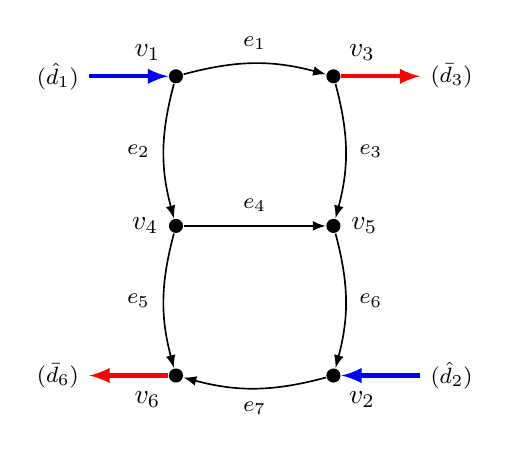
\begin{tikzpicture}[-latex ,auto,semithick,state/.style ={ draw,shape=circle,scale=0.7}]

\node[circle,fill,inner sep=1.8pt,label=above left: $v_1$] (A) at (0,0) {};
\node[circle,fill,inner sep=1.8pt,label=above right: $v_3$] (B) at (2,0) {};
\node[circle,fill,inner sep=1.8pt,label= left: $v_4$] (C) at (0,-1.9) {};
\node[circle,fill,inner sep=1.8pt,label= right: $v_5$] (D) at (2,-1.9) {};
\node[circle,fill,inner sep=1.8pt,label= below right: $v_2$] (E) at (2,-3.8) {};
\node[circle,fill,inner sep=1.8pt,label= below left: $v_6$] (F) at (0,-3.8) {};


\path (A) edge [bend right = -15] node[above  =0.05 cm] {\footnotesize$e_{1}$} (B);
\path (A) edge [bend right = 15] node[left  =0.05 cm] {\footnotesize$e_{2}$} (C);
\path (B) edge [bend right = -15] node[right  =0.05 cm] {\footnotesize$e_{3}$} (D);
\path (C) edge [bend right = 0] node[above  =0.05 cm] {\footnotesize$e_{4}$} (D);
\path (C) edge [bend right = 15] node[left  =0.05 cm] {\footnotesize$e_{5}$} (F);
\path (D) edge [bend right = -15] node[right  =0.05 cm] {\footnotesize$e_{6}$} (E);
\path (E) edge [bend right = -15] node[below  =0.05 cm] {\footnotesize$e_{7}$} (F);

\draw [-latex,line width=1.5pt,blue](-1.1,0) -- (-0.1,0);
\draw [-latex,line width=1.5pt,blue](3.1,-3.8) -- (2.1,-3.8);
\node at (-1.5,0) {\footnotesize $(\hat{d}_1)$};
\node at (3.5,-3.8) {\footnotesize $(\hat{d}_2)$};
\node at (3.5,0) {\footnotesize $(\bar{d}_3)$};
\node at (-1.5,-3.8) {\footnotesize $(\bar{d}_6)$};
\draw [-latex,line width=1.5pt,red](2.1,0) -- (3.1,0);
\draw [-latex,line width=1.5pt,red](-0.1,-3.8) -- (-1.1,-3.8);
\end{tikzpicture}
 
\vspace{2mm}
\caption{Graph of the example multi-inlet network.}
\label{fig:example1_graph}
\end{subfigure}
\begin{subfigure}{.49\textwidth}
\centering
\hspace{0mm}
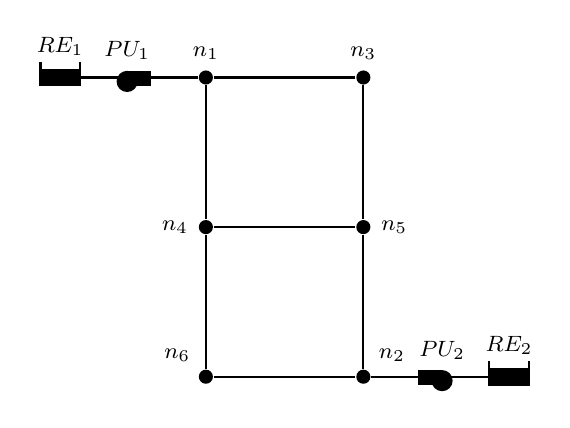
\begin{tikzpicture}[semithick,state/.style ={ draw,shape=circle,scale=0.9}]

\node[circle,fill,inner sep=1.8pt,label=above : \footnotesize$n_1$] (A) at (0,0) {};
\node[circle,fill,inner sep=1.8pt,label=above : \footnotesize$n_3$] (B) at (2,0) {};
\node[circle,fill,inner sep=1.8pt,label= left: \footnotesize$n_4$] (C) at (0,-1.9) {};
\node[circle,fill,inner sep=1.8pt,label= right: \footnotesize$n_5$] (D) at (2,-1.9) {};
\node[circle,fill,inner sep=1.8pt,label= above right: \footnotesize $n_{2}$] (E) at (2,-3.8) {};
\node[circle,fill,inner sep=1.8pt,label= above left: \footnotesize$n_6$] (F) at (0,-3.8) {};

\draw [thick] (A) --  (B) node[above  =0.05 cm] {\footnotesize$$};
\path (A) edge [thick]  node[left  =0.05 cm] {\footnotesize$$} (C);
\path (B) edge [thick] node[right  =0.05 cm] {\footnotesize$$} (D);
\path (C) edge [thick] node[above  =0.05 cm] {\footnotesize$$} (D);
\path (C) edge [thick] node[left  =0.05 cm] {\footnotesize$$} (F);
\path (D) edge [thick] node[right  =0.05 cm] {\footnotesize$$} (E);
\path (E) edge [thick] node[below  =0.05 cm] {\footnotesize$$} (F);



%PU2
\node[circle,fill,inner sep=2.7pt,label= above : \footnotesize $ PU_2$] (I) at (3,-3.85) {};
\draw [thin,fill] (2.7,-3.72) rectangle (3,-3.9);


\begin{scope}[xscale=-1,yscale=1]
%PU1
\node[circle,fill,inner sep=2.7pt,label= above : \footnotesize $ PU_1$] (I) at (3.4-2.4,-2.05+2) {};
\draw [thin,fill] (3.1-2.4,-1.92+2) rectangle (3.4-2.4,-2.1+2);

\end{scope}

\draw [thick](2.1,-3.8) -- (2.7,-3.8);
\draw [thick](-0.1,0) -- (-1.1,0);


\draw [thick](3.1,-3.8) -- (3.6,-3.8);
\draw [thick](-1.1,0) -- (-1.6,0);
\draw [thick](-1.6,0.2) -- (-1.6,-0.1) -- (-2.1,-0.1) -- (-2.1,0.2);
\draw [thick,fill] (-2.1,0.1) rectangle (-1.6,-0.1);
\draw [thick](3.6,-3.6) -- (3.6,-3.9) -- (4.1,-3.9) -- (4.1,-3.6);
\draw [thick,fill] (3.6,-3.7) rectangle (4.1,-3.9);
\node at (-1.85,0.4) {\footnotesize $RE_1$};
\node at (3.85,-3.4) {\footnotesize $RE_2$};
\end{tikzpicture} 
\vspace{3mm}
  \caption{The network in EPANET.}
  \label{fig:example_EPANET}
\end{subfigure}
\caption{The graph and EPANET model of the example network.}
\label{fig:example_sum}
\end{figure}
\vspace{-3mm}

% %Graph of example1 network
% \begin{figure}[H]
% \centering
% %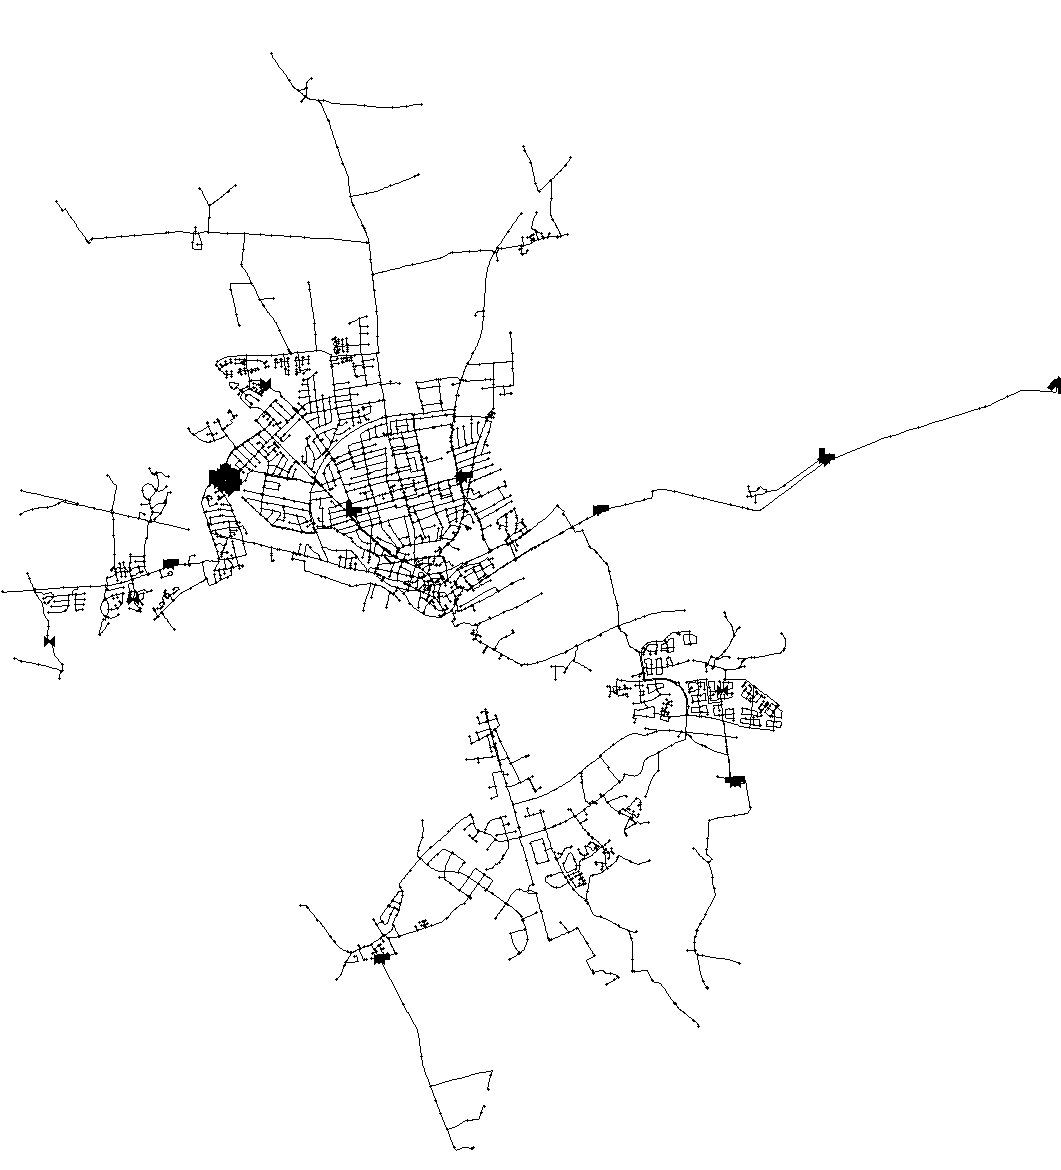
\includegraphics[width=1\textwidth]{report/pictures/verdo_pic}
% 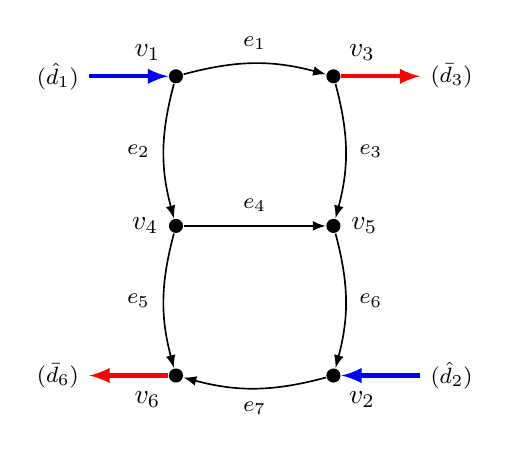
\begin{tikzpicture}[-latex ,auto,semithick,state/.style ={ draw,shape=circle,scale=0.7}]

\node[circle,fill,inner sep=1.8pt,label=above left: $v_1$] (A) at (0,0) {};
\node[circle,fill,inner sep=1.8pt,label=above right: $v_3$] (B) at (2,0) {};
\node[circle,fill,inner sep=1.8pt,label= left: $v_4$] (C) at (0,-1.9) {};
\node[circle,fill,inner sep=1.8pt,label= right: $v_5$] (D) at (2,-1.9) {};
\node[circle,fill,inner sep=1.8pt,label= below right: $v_2$] (E) at (2,-3.8) {};
\node[circle,fill,inner sep=1.8pt,label= below left: $v_6$] (F) at (0,-3.8) {};


\path (A) edge [bend right = -15] node[above  =0.05 cm] {\footnotesize$e_{1}$} (B);
\path (A) edge [bend right = 15] node[left  =0.05 cm] {\footnotesize$e_{2}$} (C);
\path (B) edge [bend right = -15] node[right  =0.05 cm] {\footnotesize$e_{3}$} (D);
\path (C) edge [bend right = 0] node[above  =0.05 cm] {\footnotesize$e_{4}$} (D);
\path (C) edge [bend right = 15] node[left  =0.05 cm] {\footnotesize$e_{5}$} (F);
\path (D) edge [bend right = -15] node[right  =0.05 cm] {\footnotesize$e_{6}$} (E);
\path (E) edge [bend right = -15] node[below  =0.05 cm] {\footnotesize$e_{7}$} (F);

\draw [-latex,line width=1.5pt,blue](-1.1,0) -- (-0.1,0);
\draw [-latex,line width=1.5pt,blue](3.1,-3.8) -- (2.1,-3.8);
\node at (-1.5,0) {\footnotesize $(\hat{d}_1)$};
\node at (3.5,-3.8) {\footnotesize $(\hat{d}_2)$};
\node at (3.5,0) {\footnotesize $(\bar{d}_3)$};
\node at (-1.5,-3.8) {\footnotesize $(\bar{d}_6)$};
\draw [-latex,line width=1.5pt,red](2.1,0) -- (3.1,0);
\draw [-latex,line width=1.5pt,red](-0.1,-3.8) -- (-1.1,-3.8);
\end{tikzpicture}
 
% \caption{Graph of a simple multi-inlet network.}
% \label{fig:example1_graph}
% \end{figure}
% \vspace{-3mm}

In \figref{fig:example1_graph}, arrows illustrate the in-and outflows such that input flows are in $v_1 $ and $v_2$ vertices, and users consume water in $v_3$ and $v_6$. The diameters are the same for all pipes, however regarding the length differ. The corresponding parameters of the pipes, pumps, the elevation profile and the hourly demand variation is described in detail and can be found in (appref). 

The partitioning of edges in this example is chosen such that

\begin{equation}
  \label{edgeorientation_example1_T}
  \mathcal{E}_{\mathcal{T}} = \{ e_1, e_5, e_3, e_4 \} \equiv \{ e_{\mathcal{T},1}, e_{\mathcal{T},2}, e_{\mathcal{T},3}, e_{\mathcal{T},4}  \},
\end{equation}

and

\begin{equation}
\label{edgeorientation_example1_C}
  \mathcal{E}_\mathcal{C} = \{e_2, e_6, e_7\} \equiv \{e_{\mathcal{C},1}, e_{\mathcal{C},2}, e_{\mathcal{C},3}\},
\end{equation}.

The corresponding vectors describing the pressures and flows in vertices and edges, respectively, furthermore the elevation and distribution profiles are given such that

\begin{equation}
\label{example1_signals_constants}
p(t) =
 \begin{pmatrix} 
 \bar{p}_3(t) \\[1.3pt] 
 \bar{p}_4(t) \\[1.3pt]
 \bar{p}_5(t) \\[1.3pt] 
 \bar{p}_6(t) \\[1.3pt] 
  \hline
 \hat{p}_1(t) \\[1.3pt] 
 \hat{p}_2(t) \\[1.3pt] 
 \end{pmatrix}
 , \hspace{5mm}
 d(t) =  \begin{pmatrix} 
 \bar{d}_3(t) \\[1pt] 
 0 \\[1pt]
 0 \\[1pt] 
 \bar{d}_6(t) \\[1pt] 
  \hline
 \hat{d}_1(t) \\[1pt] 
 \hat{d}_2(t) \\[1pt] 
 \end{pmatrix}
 , \hspace{5mm}
 h =  \begin{pmatrix} 
 \bar{h}_3 \\[1pt] 
 \bar{h}_4 \\[1pt]
 \bar{h}_5 \\[1pt] 
 \bar{h}_6 \\[1pt] 
   \hline
 0 \\[1pt] 
 0 \\[1pt] 
 \end{pmatrix}
 , \hspace{5mm}
 v =  \begin{pmatrix} 
 v_3 \\[1pt] 
 0 \\[1pt]
 0 \\[1pt] 
 v_6 \\[1pt]
 \end{pmatrix}.
\end{equation}

From this arrangement of the edges and vertices, it follows that the sub-matrix $\bar{H}_{\mathcal{T}}$ which maps non-inlet vertices to edges in set $\mathcal{E}_{\mathcal{T}}$ is invertible. 

Since there are two vertices in the system with demand, the total flow leaving the network can be written as shown in \eqref{consumption1}.

\begin{equation}
  \label{consumption1}
  \sigma(t) = -\bar{d}_3(t) - \bar{d}_6(t).
\end{equation}

By measuring the input pressures and knowing the parameters of the network, the output pressures, i.e. the pressures in the non-inlet vertices can be calculated. However, first recall \eqref{meshresult2}, 

\begin{equation}
  \label{ac_eq} 
  g(q_{\mathcal{C}}) = f_{\mathcal{C}}(q_\mathcal{C}) - A_1(\hat{p} + \hat{h}) + A_2^T f_{\mathcal{T}}(A_2 q_\mathcal{C} + A_3 \bar{d}) = 0.
\end{equation}

\begin{minipage}[t]{0.4\textwidth}
where\\
\hspace*{8mm} $A_1 = \hat{H}^T_{\mathcal{C}} -\bar{H}^T_{\mathcal{C}}\bar{H}^{-T}_{\mathcal{T}}\hat{H}^T_{\mathcal{T}}$, \vspace*{1.5mm}  \\
\hspace*{8mm} $A_2 = -\bar{H}^{-1}_{\mathcal{T}} \bar{H}_{\mathcal{C}} $, \vspace*{1.5mm}\\
\hspace*{8mm} $A_3 = \bar{H}^{-1}_{\mathcal{T}}$. 
\end{minipage}

On account of non-linearity in \eqref{ac_eq}, an analytic solution has not been found to express the flows $q_{\mathcal{C}}$. Instead, iterative numerical methods are used. As $g(q_{\mathcal{C}})$ is differentiable with respect to $q_{\mathcal{C}}$, gradient-based root finding algorithms such as Newton-Raphson method is a convenient choice \cite{woodford1997numerical}. With iterative methods, initial values of flows are repeatedly adjusted until the difference between two successive iterates is within an acceptable tolerance. Furthermore, we know from the homogeneity and monotonicity property of $g(q_{\mathcal{C}})$ that the function is a homeomorphism in $q_{\mathcal{C}}$, therefore its root must be unique. Using the gradient-based searching method, and squaring $g(q_{\mathcal{C}})$  yields

\begin{equation}
\label{gradient_search} 
  2 \frac{\partial g^T(q_{\mathcal{C}})}{\partial q_{\mathcal{C}}} g(q_{\mathcal{C}}) = 0, 
\end{equation}

By solving \eqref{gradient_search}, the unique solution is found. Furthermore, if $g^T(q_{\mathcal{C}}) g(q_{\mathcal{C}})$ is convex, the solution is the global minimum of this problem. By solving \eqref{ac_eq} for $a_{\mathcal{C}}$, the non-inlet pressures and all flows in the network can be calculated in terms of the input pressures and the total demand in the network. In order to obtain these values, the previously-derived output equation in \eqref{model_multiinlet1} is used. 

Therefore in the simulation, the most simple case is considered when the total flow demand in the network varies, however the distribution among vertices remains the same. In this case, $v$ is a constant vector, and the base demands in all vertices are the same. 

The variation curves for input pressures are the inputs both in our MATLAB implementation and in EPANET. The inlet pressures are shown in \figref{fig:sub11_example1} and the inlet flows are shown in \figref{fig:sub22_example1} for a five hour-long period.

\begin{figure}[H]
\centering
\begin{subfigure}{.49\textwidth}
\centering
  % This file was created by matlab2tikz.
%
%The latest updates can be retrieved from
%  http://www.mathworks.com/matlabcentral/fileexchange/22022-matlab2tikz-matlab2tikz
%where you can also make suggestions and rate matlab2tikz.
%
\definecolor{mycolor1}{rgb}{0.00000,0.44700,0.74100}%
\definecolor{mycolor2}{rgb}{0.85000,0.32500,0.09800}%
%
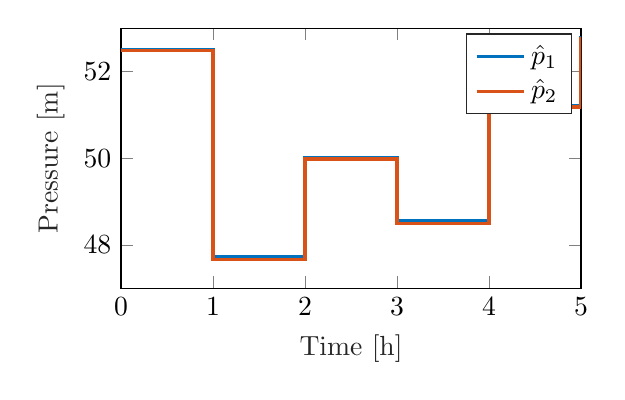
\begin{tikzpicture}

\begin{axis}[%
width=2.3in,
height=1.3in,
at={(0.766in,0.474in)},
scale only axis,
xmin=0,
xmax=5,
xlabel style={font=\color{white!15!black}},
xlabel={Time [h]},
ymin=47,
ymax=53,
ylabel style={font=\color{white!15!black}},
ylabel={Pressure [m]},
axis background/.style={fill=white},
%title style={font=\bfseries},
%title={Inlet pressures},
%xmajorgrids,
%ymajorgrids,
legend style={legend cell align=left, align=left, draw=white!15!black}
]
\addplot[const plot, color=mycolor1, line width=1.2pt] table[row sep=crcr] {%
0	52.51\\
1	47.74\\
2	50.02\\
3	48.57\\
4	51.22\\
5	52.81\\
};
\addlegendentry{$\hat{p}_1$}

\addplot[const plot, color=mycolor2, line width=1.2pt] table[row sep=crcr] {%
0	52.49\\
1	47.66\\
2	49.98\\
3	48.5\\
4	51.18\\
5	52.8\\
};
\addlegendentry{$\hat{p}_2$}

\end{axis}
\end{tikzpicture}% 
  \caption{Inlet pressures $\hat{p}$}
  \label{fig:sub11_example1}
\end{subfigure}
\begin{subfigure}{.49\textwidth}
\centering
  % This file was created by matlab2tikz.
%
%The latest updates can be retrieved from
%  http://www.mathworks.com/matlabcentral/fileexchange/22022-matlab2tikz-matlab2tikz
%where you can also make suggestions and rate matlab2tikz.
%
\definecolor{mycolor1}{rgb}{0.00000,0.44700,0.74100}%
\definecolor{mycolor2}{rgb}{0.85000,0.32500,0.09800}%
%
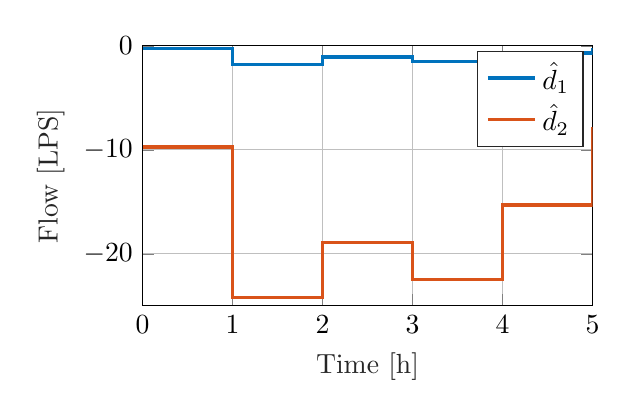
\begin{tikzpicture}

\begin{axis}[%
width=2.25in,
height=1.3in,
at={(0.791in,0.461in)},
scale only axis,
xmin=0,
xmax=5,
xlabel style={font=\color{white!15!black}},
xlabel={Time [h]},
ymin=-25,
ymax=0,
ylabel style={font=\color{white!15!black}},
ylabel={Flow [LPS]},
axis background/.style={fill=white},
%title style={font=\bfseries},
%title={Inlet demands},
xmajorgrids,
ymajorgrids,
legend style={legend cell align=left, align=left, draw=white!15!black}
]
\addplot[const plot, color=mycolor1, line width=1.2pt] table[row sep=crcr] {%
0	-0.27002029288415\\
1	-1.78959208760883\\
2	-1.07885170290758\\
3	-1.53102470893297\\
4	-0.688152757407579\\
5	-0.175509754602786\\
};
\addlegendentry{$\hat{d}_1$}

\addplot[const plot, color=mycolor2, line width=1.2pt] table[row sep=crcr] {%
0	-9.72997970711585\\
1	-24.2104079123912\\
2	-18.9211482970924\\
3	-22.468975291067\\
4	-15.3118472425924\\
5	-7.82449024539721\\
};
\addlegendentry{$\hat{d}_2$}

\end{axis}
\end{tikzpicture}% 
  \caption{Absolute value of the inlet flows $\hat{d}$}
  \label{fig:sub22_example1}
\end{subfigure}
\caption{Signals describing the input pressures(left) and flows(right) of the two pumping stations.}
\label{fig:inlet_pressures_demands}
\end{figure}

\begin{figure}[H]
\centering
\begin{subfigure}{.49\textwidth}
\centering
  % This file was created by matlab2tikz.
%
%The latest updates can be retrieved from
%  http://www.mathworks.com/matlabcentral/fileexchange/22022-matlab2tikz-matlab2tikz
%where you can also make suggestions and rate matlab2tikz.
%
\definecolor{mycolor1}{rgb}{0.00000,0.44700,0.74100}%
\definecolor{mycolor2}{rgb}{0.85000,0.32500,0.09800}%
%
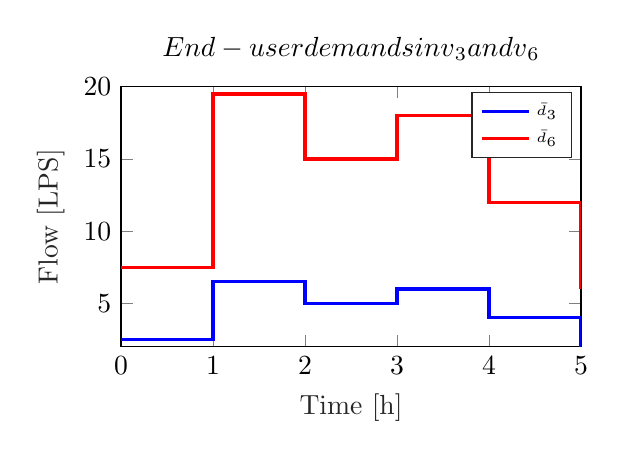
\begin{tikzpicture}

\begin{axis}[%
width=2.3in,
height=1.3in,
at={(0.758in,0.481in)},
scale only axis,
xmin=0,
xmax=5,
xlabel style={font=\color{white!15!black}},
xlabel={Time [h]},
ymin=2,
ymax=20,
ylabel style={font=\color{white!15!black}},
ylabel={Flow [LPS]},
axis background/.style={fill=white},
title style={},
title={$\text{End-user demands in v}_\text{3}\text{ and v}_\text{6}$},
%xmajorgrids,
%ymajorgrids,
legend style={legend cell align=left, align=left, draw=white!15!black}
]
\addplot[const plot, color=blue, line width=1.2pt] table[row sep=crcr] {%
0	2.5\\
1	6.5\\
2	5\\
3	6\\
4	4\\
5	2\\
};
\addlegendentry{\tiny $\bar{d}_3$}

\addplot[const plot, color=red, line width=1.2pt] table[row sep=crcr] {%
0	7.5\\
1	19.5\\
2	15\\
3	18\\
4	12\\
5	6\\
};
\addlegendentry{\tiny $\bar{d}_6$}

\end{axis}
\end{tikzpicture}% 
  \caption{Non-inlet demands $\bar{d}$}
  \label{fig:sub21_example1}
\end{subfigure}
\begin{subfigure}{.49\textwidth}
\centering
  % This file was created by matlab2tikz.
%
%The latest updates can be retrieved from
%  http://www.mathworks.com/matlabcentral/fileexchange/22022-matlab2tikz-matlab2tikz
%where you can also make suggestions and rate matlab2tikz.
%
\definecolor{mycolor1}{rgb}{0.00000,0.44700,0.74100}%
\definecolor{mycolor2}{rgb}{0.85000,0.32500,0.09800}%
\definecolor{mycolor3}{rgb}{0.92900,0.69400,0.12500}%
\definecolor{mycolor4}{rgb}{0.49400,0.18400,0.55600}%
%
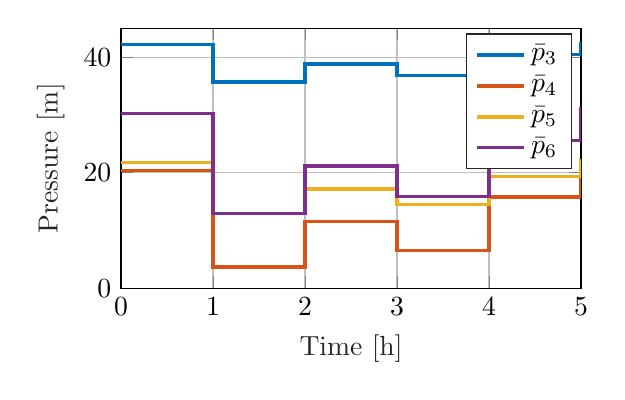
\begin{tikzpicture}

\begin{axis}[%
width=2.3in,
height=1.3in,
at={(0.758in,0.481in)},
scale only axis,
xmin=0,
xmax=5,
xlabel style={font=\color{white!15!black}},
xlabel={Time [h]},
ymin=0,
ymax=45,
ylabel style={font=\color{white!15!black}},
ylabel={Pressure [m]},
axis background/.style={fill=white},
%title style={font=\bfseries},
%title={Non-inlet pressures $(\bar{p})$},
xmajorgrids,
ymajorgrids,
legend style={legend cell align=left, align=left, draw=white!15!black}
]
\addplot[const plot, color=mycolor1, line width=1.2pt] table[row sep=crcr] {%
0	42.21\\
1	35.712\\
2	38.82\\
3	36.842\\
4	40.452\\
5	42.618\\
};
\addlegendentry{$\bar{p}_3$}

\addplot[const plot, color=mycolor2, line width=1.2pt] table[row sep=crcr] {%
0	20.3672640689439\\
1	3.67476567889016\\
2	11.6071871859654\\
3	6.54234407877965\\
4	15.7956885662872\\
5	21.4335225222452\\
};
\addlegendentry{$\bar{p}_4$}

\addplot[const plot, color=mycolor3, line width=1.2pt] table[row sep=crcr] {%
0	21.7881086237316\\
1	12.9652322870728\\
2	17.1730521589117\\
3	14.4909102062663\\
4	19.3873080072803\\
5	22.3468148852399\\
};
\addlegendentry{$\bar{p}_5$}

\addplot[const plot, color=mycolor4, line width=1.2pt] table[row sep=crcr] {%
0	30.2597113346647\\
1	12.9533643088574\\
2	21.1795244882205\\
3	15.9271407367542\\
4	25.5211869947594\\
5	31.3646680673769\\
};
\addlegendentry{$\bar{p}_6$}

\end{axis}
\end{tikzpicture}% 
  \caption{Non-inlet pressures $\bar{p}$}
  \label{fig:sub22_example1}
\end{subfigure}
\caption{Signals describing the demand flows by the end-users(left) and output pressures(right).}
\label{fig:noninlet_demands_noninlet_pressures}
\end{figure}
\vspace{-3mm}

In \figref{fig:sub22_example1}, the non-inlet pressure values corresponding to the EPANET simulation are denoted with $\bar{p}_{3e}$, $\bar{p}_{4e}$, $\bar{p}_{5e}$ and $\bar{p}_{6e}$. The pressure values denoted with $\bar{p}_{3}$, $\bar{p}_{4}$, $\bar{p}_{5}$ and $\bar{p}_{6}$ denote the results of the simulation in MATLAB. 

Furthermore, \figref{fig:flows_C_T} shows the simulation results on all non-inlet flows in $\mathcal{C}$ and $\mathcal{T}$, respectively. It should be noted that negative flows correspond to wrong initial guess on the direction of the edges in the network graph. Therefore, in Matlab the calculated flows appear with a negative sign. For that reason in the figures below, the corresponding EPANET results have been flipped as well in order to compare the results. 

\begin{figure}[H]
\centering
\begin{subfigure}{.49\textwidth}
\centering
  % This file was created by matlab2tikz.
%
%The latest updates can be retrieved from
%  http://www.mathworks.com/matlabcentral/fileexchange/22022-matlab2tikz-matlab2tikz
%where you can also make suggestions and rate matlab2tikz.
%
\definecolor{mycolor1}{rgb}{0.00000,0.44700,0.74100}%
\definecolor{mycolor2}{rgb}{0.85000,0.32500,0.09800}%
\definecolor{mycolor3}{rgb}{0.92900,0.69400,0.12500}%
%
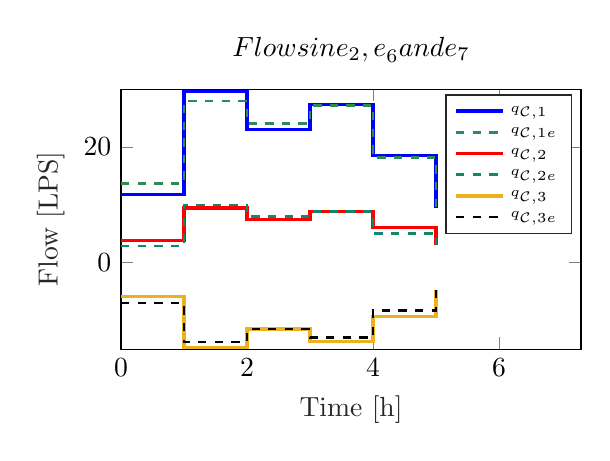
\begin{tikzpicture}

\begin{axis}[%
width=2.3in,
height=1.3in,
at={(0.758in,0.481in)},
scale only axis,
xmin=0,
xmax=7.3,
xlabel style={font=\color{white!15!black}},
xlabel={Time [h]},
ymin=-15,
ymax=30,
ylabel style={font=\color{white!15!black}},
ylabel={Flow [LPS]},
axis background/.style={fill=white},
title style={},
title={$\text{Flows in e}_\text{2}\text{, e}_\text{6}\text{ and e}_\text{7}$},
%xmajorgrids,
%ymajorgrids,
legend style={legend cell align=left, align=left, draw=white!15!black}
]
\addplot[const plot, color=blue, line width=1.2pt] table[row sep=crcr] {%
0	11.7502570959187\\
1	29.5561012463149\\
2	23.0126657096865\\
3	27.3936960334265\\
4	18.5662622910719\\
5	9.43871589453002\\
};
\addlegendentry{\tiny $q_{\mathcal{C},1}$}

\addplot[const plot, dashed, color=SeaGreen, line width=1pt] table[row sep=crcr] {%
0	13.7502570959187\\
1	27.9561012463149\\
2	24.0126657096865\\
3	27.1936960334265\\
4	18.1662622910719\\
5	8.43871589453002\\
};
\addlegendentry{\tiny $q_{\mathcal{C},1e}$}

\addplot[const plot, color=red, line width=1.2pt] table[row sep=crcr] {%
0	3.85877138476544\\
1	9.45870515475531\\
2	7.4303780100986\\
3	8.79458158128527\\
4	6.03871892954993\\
5	3.10763052781182\\
};
\addlegendentry{\tiny $q_{\mathcal{C},2}$}

\addplot[const plot, dashed, color=PineGreen, line width=1pt] table[row sep=crcr] {%
0	2.85877138476544\\
1	9.95870515475531\\
2	7.99303780100986\\
3	8.79458158128527\\
4	5.03871892954993\\
5	3.10763052781182\\
};
\addlegendentry{\tiny $q_{\mathcal{C},2e}$}

\addplot[const plot, color=mycolor3, line width=1.2pt] table[row sep=crcr] {%
0	-5.87120832235041\\
1	-14.7517027576359\\
2	-11.4907702869938\\
3	-13.6743937097818\\
4	-9.27312831304249\\
5	-4.71685971758539\\
};
\addlegendentry{\tiny $q_{\mathcal{C},3}$}

\addplot[const plot, dashed, color=black, line width=1pt] table[row sep=crcr] {%
0	-6.99120832235041\\
1	-13.7517027576359\\
2	-11.4907702869938\\
3	-12.9743937097818\\
4	-8.27312831304249\\
5	-4.71685971758539\\
};
\addlegendentry{\tiny $q_{\mathcal{C},3e}$}

\end{axis}
\end{tikzpicture}% 
  \caption{Flows in $\mathcal{C}$}
  \label{fig:sub31_example1}
\end{subfigure}
\begin{subfigure}{.49\textwidth}
\centering
  % This file was created by matlab2tikz.
%
%The latest updates can be retrieved from
%  http://www.mathworks.com/matlabcentral/fileexchange/22022-matlab2tikz-matlab2tikz
%where you can also make suggestions and rate matlab2tikz.
%
\definecolor{mycolor1}{rgb}{0.00000,0.44700,0.74100}%
\definecolor{mycolor2}{rgb}{0.85000,0.32500,0.09800}%
\definecolor{mycolor3}{rgb}{0.92900,0.69400,0.12500}%
\definecolor{mycolor4}{rgb}{0.49400,0.18400,0.55600}%
%
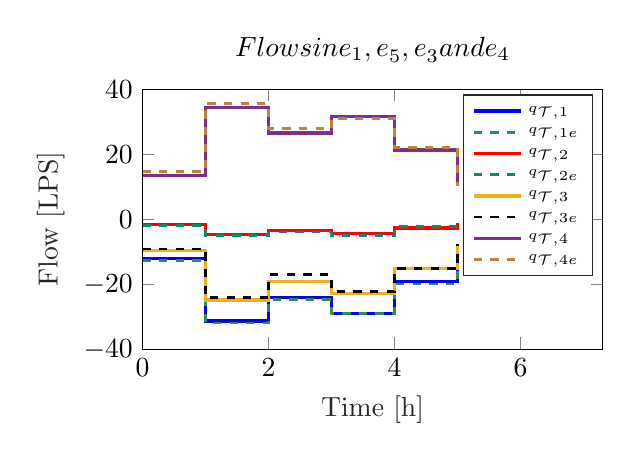
\begin{tikzpicture}

\begin{axis}[%
width=2.3in,
height=1.3in,
at={(0.758in,0.481in)},
scale only axis,
xmin=0,
xmax=7.3,
xlabel style={font=\color{white!15!black}},
xlabel={Time [h]},
ymin=-40,
ymax=40,
ylabel style={font=\color{white!15!black}},
ylabel={Flow [LPS]},
axis background/.style={fill=white},
title style={},
title={$\text{Flows in e}_\text{1}\text{, e}_\text{5}\text{, e}_\text{3}\text{ and e}_\text{4}$},
%xmajorgrids,
%ymajorgrids,
legend style={legend cell align=left, align=left, draw=white!15!black}
]
\addplot[const plot, color=blue, line width=1.2pt] table[row sep=crcr] {%
0	-12.0202773888028\\
1	-31.3456933339238\\
2	-24.0915174125941\\
3	-28.9247207423594\\
4	-19.2544150484795\\
5	-9.61422564913281\\
};
\addlegendentry{\tiny $q_{\mathcal{T},1}$}

\addplot[const plot, dashed, color=SeaGreen, line width=1pt] table[row sep=crcr] {%
0	-12.7202773888028\\
1	-31.9456933339238\\
2	-24.7915174125941\\
3	-28.9247207423594\\
4	-19.9544150484795\\
5	-9.61422564913281\\
};
\addlegendentry{\tiny $q_{\mathcal{T},1e}$}

\addplot[const plot, color=red, line width=1.2pt] table[row sep=crcr] {%
0	-1.62879167764959\\
1	-4.74829724236414\\
2	-3.50922971300619\\
3	-4.32560629021824\\
4	-2.72687168695751\\
5	-1.28314028241461\\
};
\addlegendentry{\tiny $q_{\mathcal{T},2}$}

\addplot[const plot, dashed, color=PineGreen, line width=1pt] table[row sep=crcr] {%
0	-1.92879167764959\\
1	-4.94829724236414\\
2	-3.90922971300619\\
3	-4.92560629021824\\
4	-2.12687168695751\\
5	-1.28314028241461\\
};
\addlegendentry{\tiny $q_{\mathcal{T},2e}$}

\addplot[const plot, color=mycolor3, line width=1.2pt] table[row sep=crcr] {%
0	-9.52027738880282\\
1	-24.8456933339238\\
2	-19.0915174125941\\
3	-22.9247207423594\\
4	-15.2544150484795\\
5	-7.6142256491328\\
};
\addlegendentry{\tiny $q_{\mathcal{T},3}$}

\addplot[const plot, dashed, color=black, line width=1pt] table[row sep=crcr] {%
0	-9.12027738880282\\
1	-24.1456933339238\\
2	-17.0915174125941\\
3	-22.1247207423594\\
4	-15.2544150484795\\
5	-7.6142256491328\\
};
\addlegendentry{\tiny $q_{\mathcal{T},3e}$}

\addplot[const plot, color=mycolor4, line width=1.2pt] table[row sep=crcr] {%
0	13.3790487735683\\
1	34.3043984886791\\
2	26.5218954226927\\
3	31.7193023236447\\
4	21.2931339780294\\
5	10.7218561769446\\
};
\addlegendentry{\tiny $q_{\mathcal{T},4}$}

\addplot[const plot, dashed, color=brown, line width=1pt] table[row sep=crcr] {%
0	14.5790487735683\\
1	35.5043984886791\\
2	27.9218954226927\\
3	31.1193023236447\\
4	21.9931339780294\\
5	10.1218561769446\\
};
\addlegendentry{\tiny $q_{\mathcal{T},4e}$}


\end{axis}
\end{tikzpicture}% 
  \caption{Flows in $\mathcal{T}$}
  \label{fig:sub31_example1}
\end{subfigure}
\caption{Signals describing the flows in all pipes in the network.}
\label{fig:flows_C_T}
\end{figure}
\vspace{-3mm}

From the comparison of non-inlet flows and non-inlet pressures we can see that our implementation of the Multi-inlet model in MATLAB yields the same results as in EPANET. The small difference between the pressure and flow values is due to the fact that our model does not take into account that the friction factor of pipe elements might change according to the flows.  

Therefore, the framework of modelling introduced in this section is further discussed in the following sections where we extend the current model and we include the dynamics of elevated reservoirs. 

\newpage

\section{Inclusion of elevated reservoirs}
\label{inclusion_of_reservoirs}

When a WT is being attached to an existing pipe network, certain properties of the system must be modified. Regarding the underlying graph of the network, when a WT is attached, the vertex to which the WT is connected becomes a vertex with a demand. However, the demand flow which describes the filling and emptying process of the tank, in this case, is not directly related to any user consumption profile, since flow can go into and come out of the WT. Therefore, the constraint on demand flows, previously described in \eqref{non_inlet_constraint} is not valid in case of elevated reservoirs, as this type of demand flow can be both positive or negative. For this reason, demands on the WTs are treated as inputs and added to the vertices marked with hats $\hat{p}$ and $\hat{d}$. The vertices on which demand of WTs are defined are selected from the overall inlet flows such that 

\begin{subequations}
\begin{equation}
\label{tank_inclusion_separation_of_input_demand}
\hat{d} = F \hat{d}_t + G \hat{d}_c ,
\end{equation}


 \begin{minipage}[t]{0.20\textwidth}
where\\
\hspace*{8mm} $\hat{d}_t \in \: \mathbb{R}^{l }$\\
\hspace*{8mm} $\hat{d}_c \in \: \mathbb{R}^{c }$ \\
\newline
\hspace*{6mm} $F^T \in \: \mathbb{R}^{(l\! \times \!c\!+\!l)}$ \\
\hspace*{6mm} $G^T \in \: \mathbb{R}^{(c\! \times \!c\!+\!l )}$
\end{minipage}
\begin{minipage}[t]{0.68\textwidth}
\vspace*{2mm}
is the vector of demand flows corresponding to WTs,\\
is the the vector of demand flows corresponding to the pump inlets, \\
is a mapping which selects the vertices belonging to WTs, \\
is a mapping which selects the vertices belonging to pump inlets.
\end{minipage}

The same partitioning is done for the input pressures and elevation, regarding pumps and WTs.

\begin{equation}
\label{tank_inclusion_separation_of_input_pressure_elevation1}
\hat{h} = F \hat{h}_t + G \hat{h}_c, 
\end{equation}
\vspace{-3mm}

\begin{equation}
\label{tank_inclusion_separation_of_input_pressure_elevation2}
\hat{p} = F \hat{p}_t + G \hat{p}_c,
\end{equation}

\end{subequations}

 \begin{minipage}[t]{0.20\textwidth}
where\\
\hspace*{8mm} $\hat{h}_t \in \: \mathbb{R}^{l }$\\
\hspace*{8mm} $\hat{h}_c \in \: \mathbb{R}^{c }$ \\
\newline
\hspace*{8mm} $\hat{p}_t \in \: \mathbb{R}^{l }$\\
\hspace*{8mm} $\hat{p}_c \in \: \mathbb{R}^{c }$ 
\end{minipage}
\begin{minipage}[t]{0.68\textwidth}
\vspace*{2mm}
is the vector of the elevation of the WTs,\\
is the the vector of the elevation of the pump stations,\\
is the vector of the absolute pressures in the WTs,\\
is the vector of the absolute pump inlet pressures.
\end{minipage}

With the inclusion of WTs, the network is not only constrained by the static relation between pressure and flow, as in case of the previously-derived model without WTs, but also governed by the dynamic equation describing the WT. These dynamics act as integrators on the flows $\hat{d}_t$ which go in or out of the tank. In terms of $\hat{d}_t$, the dynamics of the tanks set the pressure contribution $\hat{p}_t$ , as an input to the WSS. The block diagram of such system is shown in \figref{fig:WT_system_blockdiagram}.

%Pumping stations and waterworks in Randers
\begin{figure}[H]
\centering
%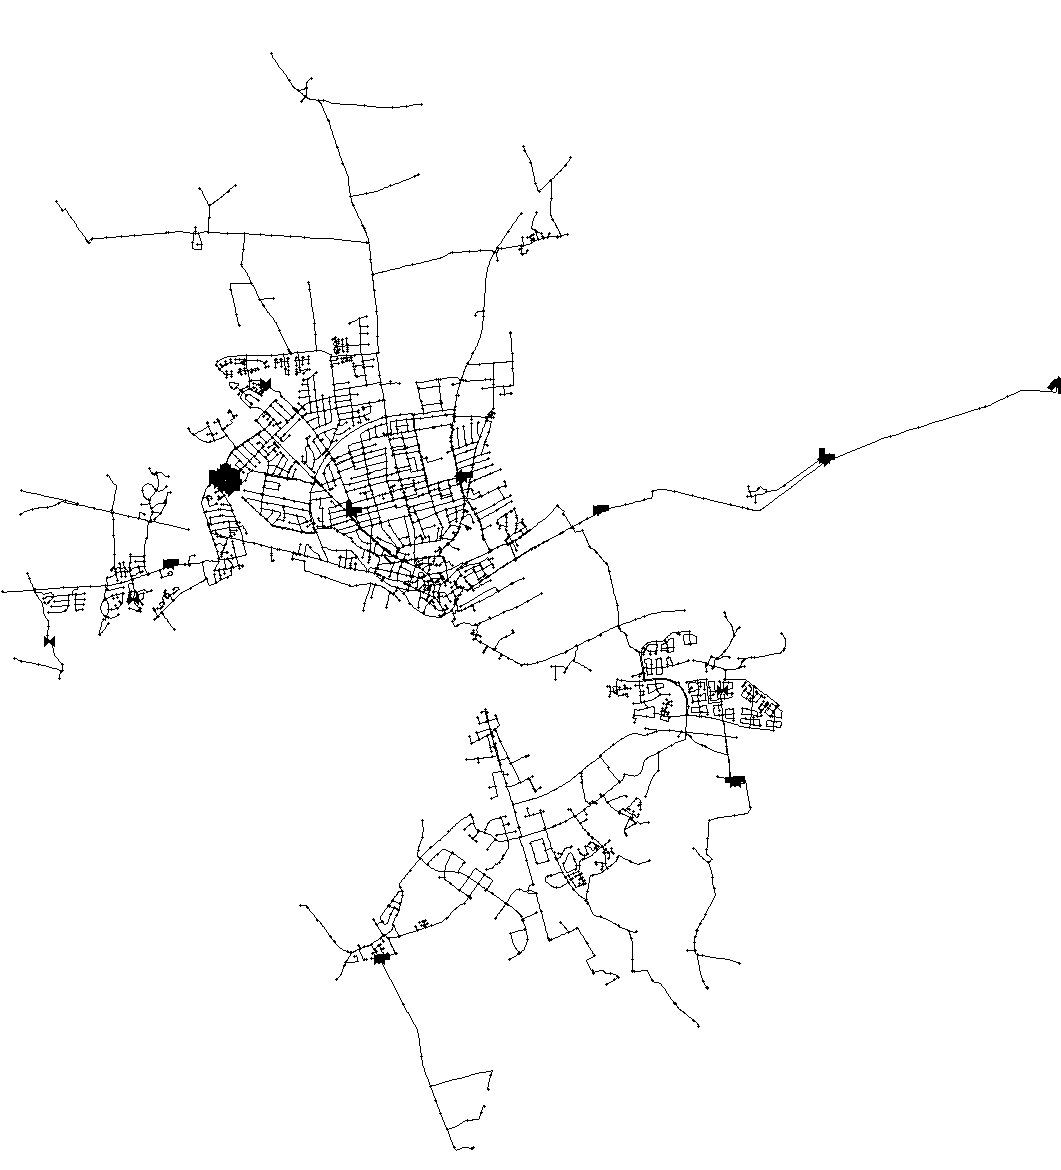
\includegraphics[width=1\textwidth]{report/pictures/verdo_pic}
 \usetikzlibrary{arrows}
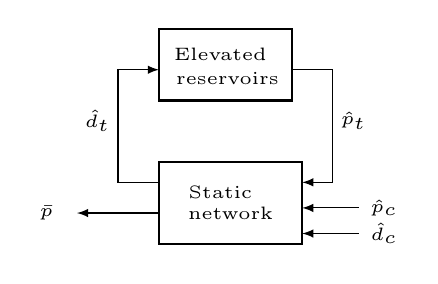
\begin{tikzpicture}[scale=1.3,transform shape]

\node at (-1.2,-2.5) {\tiny Static};
\node at (-1.1,-2.7) {\tiny network};
\node at (-1.2,-1.15) {\tiny Elevated};
\node at (-1.13,-1.38) {\tiny reservoirs};
\node at (0.1,-1.8) {\tiny $\hat{p}_t$};
\node at (-2.4,-1.8) {\tiny $\hat{d}_t$};
\node at (0.4,-2.65) {\tiny $\hat{p}_c$};
\node at (0.4,-2.9) {\tiny $\hat{d}_c$};
\node at (-2.9,-2.7) {\tiny $\bar{p}$};

\draw [thick] (-1.8,-0.9) rectangle (-0.5,-1.6);
\draw [thick] (-1.8,-2.2) rectangle (-0.4,-3);
\draw [-latex](-0.5,-1.3) -- (-0.1,-1.3) -- (-0.1,-2.4) -- (-0.4,-2.4);
\draw [-latex](0.15,-2.65) -- (-0.4,-2.65);
\draw [-latex](0.15,-2.9) -- (-0.4,-2.9);
\draw [-latex](-1.8,-2.4) -- (-2.2,-2.4) -- (-2.2,-1.3) -- (-1.8,-1.3);
\draw [-latex](-1.8,-2.7) -- (-2.6,-2.7);
\end{tikzpicture} 
\caption{Block diagram of the system extended with WTs.}
\label{fig:WT_system_blockdiagram}
\end{figure}
\vspace{-3mm}

where the 'Elevated reservoirs' block represents the subsystem with dynamics, and the 'Static network' subsystem is governed by the algebraic flow and pressure relations which describe flow and pressure in the whole pipe network. 

When elevated reservoirs are introduced in the network, the system usually operates such that the control inputs are the flows $\hat{d}$, as this is the most practical and robust way to control the network. In fact, this is the case regarding the Randers WSS, as the two pumping stations which are filling the tanks are controlled by flow, as it has been explained in \secref{waterworks_and_pumping_stations}. Therefore, the modelling approach we are about to present is different from what is handled in case of a network without a WT, since instead of using the pressures $\hat{p}$, the inlet flows $\hat{d_c}$ are considered as inputs to the model. Furthermore, regarding the dynamics, the filling and emptying process of a tank is dependent on how much flow is delivered by the pumps. This inlet flow in general is provided by multiple pumping stations, however, we make a distinction between single and multiple-WT  networks. In the former case, the flows delivered by the pumps are filling or emptying the one and only tank in the network. In the latter case, the model needs to be able to handle the flow distribution among the different WTs, meaning that different pumping stations can have different filling or emptying effects on the WTs. Therefore, in the further discussion first the case with one WT is presented, then multiple-WTs are considered.


\section{Multi-inlet/single-WT model}
\label{multi_inlet_single_WT_model}

Recalling the dynamics of one WT, in \eqref{wt_model2}, we can write the following in \eqref{wt_model_demand1}.

\begin{equation}
\label{wt_model_demand1}
\dot{\hat{p}}_{t} = -\tau \hat{d}_{t},
\end{equation}
\vspace{-3mm}

 \begin{minipage}[t]{0.20\textwidth}
where\\
\hspace*{8mm} $\hat{d}_t  \in \: \mathbb{R}$ \\
\hspace*{8mm} $\tau  \in \: \mathbb{R_{+}}$
\end{minipage}

From \eqref{wt_model_demand1} we can see that the flow $\hat{d}_t$, needs to be expressed in terms of the inputs $\hat{d}_c$. In order to express the demand regarding the WT, the whole network is treated as one vertex, as illustrated in \figref{fig:onenode_system}. 

 %Network illustration as one node
\begin{figure}[H]
\centering
%
\includegraphics[width=0.35\textwidth]{report/pictures/missingfigure}
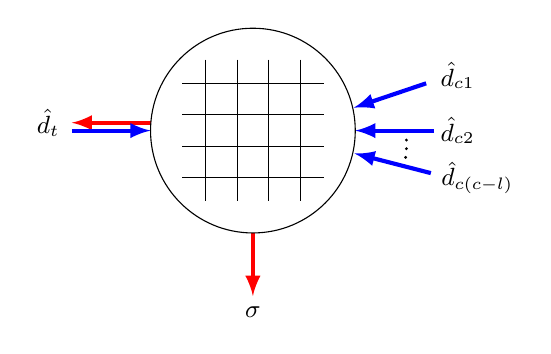
\begin{tikzpicture}[scale=1,transform shape]

\draw [-latex,line width=1.5pt,red](-0.3,-1.9) -- (-0.3,-2.7);
\draw [-latex,line width=1.5pt,blue](2,-0.6) -- (1,-0.6);
\draw [-latex,line width=1.5pt,blue](1.9,0) -- (0.98,-0.31);
\draw [-latex,line width=1.5pt,red](-1.6,-0.5) -- (-2.6,-0.5);
\draw [-latex,line width=1.5pt,blue](-2.6,-0.6) -- (-1.6,-0.6);
\draw [-latex,line width=1.5pt,blue](1.96,-1.14) -- (0.99,-0.89);

\draw (-0.9,0.3) -- (-0.9,-1.5);
\draw (-0.5,0.3) -- (-0.5,-1.5);
\draw (-0.1,0.3) -- (-0.1,-1.5);
\draw (0.3,0.3) -- (0.3,-1.5);
\draw (-1.2,0) -- (0.6,0);
\draw (-1.2,-0.4) -- (0.6,-0.4);
\draw (-1.2,-0.8) -- (0.6,-0.8);
\draw (-1.2,-1.2) -- (0.6,-1.2);
\draw  (-0.3,-0.6) ellipse (1.3 and 1.3);

\node at (2.3,0.1) {\small $\hat{d}_{c1}$};
\node at (2.3,-0.6) {\small $\hat{d}_{c2}$};
\node at (2.55,-1.2) {\small $\hat{d}_{c(c-l)}$};
\node at (-2.9,-0.5) {\small $\hat{d}_t$};
\node at (-0.3,-2.9) {\small $\sigma$};

\node[circle,fill,inner sep=0.4pt] (A) at (1.65,-0.72) {};
\node[circle,fill,inner sep=0.4pt] (A) at (1.64,-0.94) {};
\node[circle,fill,inner sep=0.4pt] (A) at (1.65,-0.83) {};

\end{tikzpicture} 
\caption{Mass balance on the network with one WT.}
\label{fig:onenode_system}
\end{figure}
\vspace{-3mm}

According to the mass-balance in the network, and using the corresponding partitioning as shown in \figref{fig:onenode_system}, the balance equation on all demand flows can be written as shown in \eqref{massbalance_model2}.

\begin{equation}
\label{massbalance_model2}
1^Td 
 =
 1^T
\begin{pmatrix} 
\bar{d} \\
\hat{d}
\end{pmatrix}
=
1^T
\begin{pmatrix} 
-v \sigma \\
\hat{d}_c \\
\hat{d}_t 
\end{pmatrix}
=
0
\end{equation}

Now, expressing $\hat{d}_t $ from \eqref{massbalance_model2} yields

\begin{equation}
\label{massbalance_model2_1}
\hat{d}_t  = \sigma - 1^T \hat{d}_c,
\end{equation}

where it is shown that if the control flows $\hat{d}_c$, are higher than the total consumption $\sigma$, the WT is being filled. The WT is being emptied if $\hat{d}_c$ is lower than $\sigma$. Thus, the system dynamics can be reformulated such that

\begin{equation}
\label{wt_model_demandd}
\dot{\hat{p}}_t = -\tau (\sigma - 1^T \hat{d}_c).
\end{equation}

It is important to point out that this first-order ODE in \eqref{wt_model_demandd} describes the mass-balance model of a single-WT system, where the input flows equal to the overall demand in the network and the rate of change of the stored water in the tank. The result is not surprising, since according to \eqref{wt_model_demandd}, the water level or equivalently the pressure fluctuates according to the in- and outflow of water, which corresponds to the pumping effort and demand in the network. 

In the single-WT modelling case, the dynamics can be described by a one-state, scalar equation, however the model is restricted to only one WT. As shown before, we know that this is not the case in the Randers WSS. Therefore, a more general description of the network is required, without restriction on the number of elevated reservoirs. 

In case of the single-WT model, the outputs are the inlet pressures of the $c$ pumping stations. During the derivation of such model, several issues have been faced due to the presence of the constraint on the network set by $q_{\mathcal{C}}$ flows. With this type of modelling, it proved to be difficult to express a model which is suitable for control purposes. Therefore, during the derivation of the general case, we attempt to use a different approaches than writing up mass-balance for the whole network.  

\section{Multi-inlet/multi-WT model}
\label{multi_inlet_multi_WT_model}

In case there are more than one WTs, the model based on the mass-balance equation proposed in \eqref{massbalance_model2} is not applicable. This is due to the fact that the inlet pressures have to be balanced, similarly as in a simple connected-volume system. Therefore, a slightly different modelling approach is required which can handle the dynamics of multiple WTs, constrained by the static network and driven by the inlet flows of the pumping stations. In order to derive such a model, the partitioning of the network is reconsidered. As described previously, the incidence matrix is partitioned such that 

\begin{equation}
\label{H_matrix_sub1}
H=
\begin{pmatrix}
\bar{H}_{\mathcal{T}} & \bar{H}_{\mathcal{C}} \\[3pt]
\hat{H}_{\mathcal{T}} & \hat{H}_{\mathcal{C}}
\end{pmatrix},
\end{equation}

where $\bar{H}_{\mathcal{T}}$ is invertible. The partitioning rule on the edges is kept from before, however in the following model description we let us slightly modify the notation and partitioning of the vertices. Now let

\begin{equation}
  \label{vertices1_1}
  \mathcal{V} = \{\bar{\mathcal{V}}, \hat{\mathcal{V}} \}, 
\end{equation}

\begin{minipage}[t]{0.3\textwidth}
where\\
\hspace*{8mm} $\hat{\mathcal{V}} = \{\hat{v}_1, ..., \hat{v}_l\}$\\
\newline
and \\
\hspace*{8mm} $\bar{\mathcal{V}} = \{\bar{v}_1, ..., \bar{v}_{n-l}\}$ 
\end{minipage}
\begin{minipage}[t]{0.67\textwidth}
\vspace*{2mm}
 represents the vertices corresponding to the points where WTs are connected,\\
 \newline
 represents the remaining vertices in the graph.
\end{minipage}

We originally defined $\bar{d}$ to describe non-inlet demands in the network and $\hat{d}$ to describe inlet-flows of the pumping stations, along with the demands of the WTs. With the redefined notation and partitioning rule on the vertices, we make sure that the vertices related to tanks are in the set $\hat{\mathcal{V}}$ and all other points in the network are in $\bar{\mathcal{V}}$. Therefore now, $\hat{d}$ describes flows regarding the WTs. In order to express the controlled inlet and non-inlet points in the network, the vectors related to $\bar{\mathcal{V}}$, namely $\bar{p}$ and $\bar{d}$, are further partitioned such that

\begin{subequations}

\begin{equation}
\label{barequation_sep1}
\bar{p} = K \bar{p}_{\mathcal{K}} + D \bar{p}_{\mathcal{D}}, 
\end{equation}

\vspace{-2mm}

\begin{equation}
\label{barequation_sep2}
\bar{d} = K \bar{d}_{\mathcal{K}} + D \bar{d}_{\mathcal{D}},  
\end{equation}

\end{subequations}

 \begin{minipage}[t]{0.3\textwidth}
where\\
\hspace*{8mm} $\bar{p}_{\mathcal{K}}$ \\
\hspace*{8mm} $\bar{p}_{\mathcal{D}}$  \\
\hspace*{8mm} $\bar{d}_{\mathcal{K}}$ \\
\hspace*{8mm} $\bar{d}_{\mathcal{D}} = -v_{\mathcal{D}} \sigma$  \\
\hspace*{8mm} $K^T \in  \mathbb{R}^{(c  \times n-l)}$ \\
\hspace*{8mm} $D^T \in  \mathbb{R}^{(n-l-c  \times n-l)}$
\end{minipage}
\begin{minipage}[t]{0.68\textwidth}
\vspace*{2mm}
is the vector of the inlet pressures ,\\
is the vector of the non-inlet pressures, \\
is the vector of the controlled inlet flows, \\
is the vector of the non-inlet demands, \\
is a mapping which selects vertices which belong to the inlets, \\
is a mapping which selects the remaining vertices.
\end{minipage}

With this partitioning of the vertices, similarly to the model presented in \secref{multi_inlet_reduced_network_description}, Kirchhoff's and Ohm's law is formulated. Recalling Kirchhoff's vertex law yields

\begin{equation}
\label{kirchhoffslaw_matrix}
\begin{pmatrix}
   \bar{H}^T_{\mathcal{T}} & \hat{H}^T_{\mathcal{T}} \\[3pt]
   \bar{H}^T_{\mathcal{C}} & \hat{H}^T_{\mathcal{C}} 
   \end{pmatrix}
 \begin{pmatrix} 
 q_\mathcal{T} \\[3pt]
 q_\mathcal{C} 
 \end{pmatrix}
 =
\begin{pmatrix} 
 \bar{d}  \\[3pt] 
 \hat{d}  
 \end{pmatrix},
\end{equation}

and recalling \eqref{ohmslaw_matrixform}, Ohm's law is given such that

\begin{equation}
\label{ohmslaw_matrixform11}
 \begin{pmatrix} 
 f_{\mathcal{T}}(q_\mathcal{T}) \\[3pt]
 f_{\mathcal{C}}(q_\mathcal{C}) 
 \end{pmatrix}
 =
 \begin{pmatrix}
   \bar{H}^T_{\mathcal{T}} & \hat{H}^T_{\mathcal{T}} \\[3pt]
   \bar{H}^T_{\mathcal{C}} & \hat{H}^T_{\mathcal{C}} 
   \end{pmatrix}
   \begin{pmatrix} 
 \bar{p} + \bar{h} \\[3pt] 
 \hat{p} + \hat{h} 
 \end{pmatrix}.
\end{equation}

In order to get an expression for $\hat{d}$, describing the flows regarding the WTs, lets define matrix $\Omega$ as follows:

\begin{equation}
\label{omega_matrix}
\Omega
=
\begin{pmatrix} 
 -\hat{H}_{\mathcal{T}}  \bar{H}^{-1}_{\mathcal{T}}  & I  
 \end{pmatrix}.
\end{equation}

Multiplying \eqref{kirchhoffslaw_matrix} with $\Omega$ from the left-hand side, $\hat{d}$ can be expressed such that

\begin{equation}
\label{WT_flows}
\hat{d} = (\hat{H}_{\mathcal{C}} - \hat{H}_{\mathcal{T}} \bar{H}^{-1}_{\mathcal{T}}\bar{H}_{\mathcal{C}})  q_\mathcal{C}  + \hat{H}_{\mathcal{T}} \bar{H}^{-1}_{\mathcal{T}} \bar{d}.
\end{equation}

As shown in \eqref{WT_flows}, the vertex law describes the dependencies of the WT demands on $\bar{d}$, which now consists of the inlet pump flows and the non-inlet demands in the rest of the network, and also shows the dependencies on $q_\mathcal{C}$. Recalling and rewriting the equation governing elevated reservoirs in matrix form, we can write the following

\begin{equation}
\label{WT_matrixform}
\Lambda \dot{\hat{p}} = - \hat{d},
\end{equation}

where $\Lambda = diag(\frac{1}{\tau_1},... ,\frac{1}{\tau_l}) \in \: \mathbb{R}^{l \times l} \succ 0$. 

In \eqref{WT_matrixform} SI units are considered for the pressures. However, if we make the conversion to pressure head, the diagonal matrix $\Lambda$ simplifies to:
$\Lambda = diag(A_{wt,1},... ,A_{wt,l}) \in \: \mathbb{R}^{l \times l} \succ 0$. 

Continuing the derivation and inserting $\hat{d}$ in \eqref{WT_flows}, into \eqref{WT_matrixform} leads to

\begin{equation}
\label{WT_matrixform_1}
\Lambda \dot{\hat{p}} = - (\hat{H}_{\mathcal{C}} - \hat{H}_{\mathcal{T}} \bar{H}^{-1}_{\mathcal{T}}\bar{H}_{\mathcal{C}})  q_\mathcal{C}  - \hat{H}_{\mathcal{T}} \bar{H}^{-1}_{\mathcal{T}} \bar{d}.
\end{equation}

Now, with the partitioning of $\bar{d}$, the inlet and non-inlet demands are inserted into \eqref{WT_matrixform_1}, resulting in the governing expression of the WT dynamics

\begin{equation}
\label{WT_matrixform_final}
\Lambda \dot{\hat{p}} = - (\hat{H}_{\mathcal{C}} - \hat{H}_{\mathcal{T}} \bar{H}^{-1}_{\mathcal{T}}\bar{H}_{\mathcal{C}})  q_\mathcal{C}  - \hat{H}_{\mathcal{T}} \bar{H}^{-1}_{\mathcal{T}} K \bar{d}_{\mathcal{K}} + \hat{H}_{\mathcal{T}} \bar{H}^{-1}_{\mathcal{T}} D v_{\mathcal{D}} \sigma .
\end{equation}

As shown in \eqref{WT_matrixform_final}, the dynamics are now in terms of the inputs $\bar{d}_{\mathcal{K}}$, the overall demand in the network $\sigma$ and $q_\mathcal{C}$. Recalling \eqref{meshresult2} in \secref{multi_inlet_reduced_network_description} and using the abbreviations for the corresponding matrices, Ohm's law has been reformulated such that

 \begin{equation}
\label{meshresult2_WT_model}
f_{\mathcal{C}}(q_\mathcal{C}) -A_1(\hat{p} + \hat{h}) + A_2^T f_{\mathcal{T}}(A_2 q_\mathcal{C} + A_3 \bar{d}) = 0.
\end{equation} 

\begin{minipage}[t]{0.4\textwidth}
where\\
\hspace*{8mm} $A_1 = \hat{H}^T_{\mathcal{C}} -\bar{H}^T_{\mathcal{C}}\bar{H}^{-T}_{\mathcal{T}}\hat{H}^T_{\mathcal{T}}$, \vspace*{1.5mm}  \\
\hspace*{8mm} $A_2 = -\bar{H}^{-1}_{\mathcal{T}} \bar{H}_{\mathcal{C}} $, \vspace*{1.5mm}\\
\hspace*{8mm} $A_3 = \bar{H}^{-1}_{\mathcal{T}}$. 
\end{minipage}

Now, using again that $\bar{d} = K \bar{d}_{\mathcal{K}} + D \bar{d}_{\mathcal{D}}$, the following implicit expression yields which allows us to calculate $q_\mathcal{C}$

 \begin{equation}
\label{meshresult2_WT_model1}
f_{\mathcal{C}}(q_\mathcal{C}) - A_1(\hat{p} + \hat{h}) + A_2^T f_{\mathcal{T}}(A_2 q_\mathcal{C} + A_3 K \bar{d}_{\mathcal{K}} - A_3 D v_{\mathcal{D}} \sigma) = 0.
\end{equation} 

Along with the implicit expression for $q_\mathcal{C}$ in \eqref{meshresult2_WT_model1}, \eqref{WT_matrixform_final} describes the dynamics of the system, taking into account the static constraints by the demands. Therefore, the structure of the overall Multi-inlet, multi-WT model dynamics can be summarized as shown in \eqref{final_flowmodel}.

\begin{equation}
\label{final_flowmodel}
\begin{cases}
    \Lambda \dot{\hat{p}}(t) = - (\hat{H}_{\mathcal{C}} - \hat{H}_{\mathcal{T}} \bar{H}^{-1}_{\mathcal{T}}\bar{H}_{\mathcal{C}})  q_\mathcal{C}(t)  - \hat{H}_{\mathcal{T}} \bar{H}^{-1}_{\mathcal{T}} K \bar{d}_{\mathcal{K}}(t) + \hat{H}_{\mathcal{T}} \bar{H}^{-1}_{\mathcal{T}} D v_{\mathcal{D}}(t) \sigma(t), \vspace{2mm}\\
    f_{\mathcal{C}}(q_\mathcal{C}(t)) - A_1(\hat{p}(t) + \hat{h}) + A_2^T f_{\mathcal{T}}(A_2 q_\mathcal{C}(t) + A_3 K \bar{d}_{\mathcal{K}}(t) - A_3 D v_{\mathcal{D}}(t) \sigma(t)) = 0.
\end{cases}
\end{equation}

\eqref{final_flowmodel} is a system of first-order ODEs with a constraint, specifying how the system evolves in time, given initial values of the states $\hat{p}$, the inputs $\bar{d}_{\mathcal{K}}$, and parametrized by the time-varying parameter $v_{\mathcal{D}}$. The constraint which is given by the algebraic equations regarding the static network, defines the manifold on which the trajectory of the ODE solution can be found. 

The states of the system are the pressures in the WTs. Therefore, when the model equations are solved for $q_\mathcal{C}$, initial information of the pressure values, $\hat{p}$ is required. Equivalently, the initial water levels in the tanks have to be known, as for any ODE. Furthermore, the initial value should be inside the set described by the algebraic constraint. 

In order to calculate the corresponding pressure inputs $\bar{p}_{\mathcal{K}}$, first $\bar{p}$ is expressed from Ohm's law as proposed in \secref{multi_inlet_reduced_network_description}.

\begin{equation}
  \label{non-inlet_p_WT}
  \bar{p} =  \bar{H}^{-T}_{\mathcal{T}}f_{\mathcal{T}}(-\bar{H}^{-1}_{\mathcal{T}} \bar{H}_{\mathcal{C}} q_\mathcal{C} + \bar{H}^{-1}_{\mathcal{T}} \bar{d}) - \bar{H}^{-T}_{\mathcal{T}}\hat{H}^{T}_{\mathcal{T}} (\hat{p} + \hat{h}) - \bar{h} .
\end{equation}

Now using that $\bar{p}_{\mathcal{K}} = K^T \bar{p} $, the pressure input equation becomes:

\begin{equation}
  \label{non-inlet_p_WT1}
  \bar{p}_{\mathcal{K}} = K^T \bar{H}^{-T}_{\mathcal{T}}f_{\mathcal{T}}(A_2 q_\mathcal{C} + A_3 K \bar{d}_{\mathcal{K}} - A_3 D v_{\mathcal{D}} \sigma) - K^T\bar{H}^{-T}_{\mathcal{T}}\hat{H}^{T}_{\mathcal{T}} (\hat{p} + \hat{h}) - K^T\bar{h} .
\end{equation}

Furthermore, using that $\bar{p}_{\mathcal{D}} = D^T \bar{p} $, the pressure output equation yields:

\begin{equation}
  \label{non-inlet_p_WT111}
  \bar{p}_{\mathcal{D}} = D^T \bar{H}^{-T}_{\mathcal{T}}f_{\mathcal{T}}(A_2 q_\mathcal{C} + A_3 K \bar{d}_{\mathcal{K}} - A_3 D v_{\mathcal{D}} \sigma) - D^T\bar{H}^{-T}_{\mathcal{T}}\hat{H}^{T}_{\mathcal{T}} (\hat{p} + \hat{h}) - D^T\bar{h}.
\end{equation}

Equivalently, \eqref{final_flowmodel} and \eqref{non-inlet_p_WT111} can be described in a more abstract form, considering a non-linear State-Space(SS) system structure such that

\begin{equation}
\label{final_flowmodel_abstract}
\begin{cases}
    \dot{\hat{p}} = g_{v_{\mathcal{D}}}( \bar{d}_{\mathcal{K}}, \sigma, q_\mathcal{C})\\
    \bar{p}_{\mathcal{K}} =h_{v_{\mathcal{D}}}(\hat{p}, \bar{d}_{\mathcal{K}}, \sigma, q_\mathcal{C})
\end{cases}
\end{equation}
\begin{equation*}
s.t. \:\:\:\:\: q_\mathcal{C} = q_\mathcal{C}((\hat{p}+\hat{h}), \bar{d}_{\mathcal{K}}, \sigma)
\end{equation*}

with $\hat{p} \in \mathbb{R}^{l}$ the state vector, $\bar{d}_{\mathcal{K}} \in \mathbb{R}^{c}$ the input vector, $\sigma \in \mathbb{R}_{+}$ the measurable disturbance, $v_{\mathcal{D}} \in \mathbb{R}^{(n-l-c)}$ the time-varying distribution parameter and $\bar{p}_{\mathcal{K}} \in \mathbb{R}^{c}$ the output vector. 

Although the ODE describing the dynamics is linear, the output and constraint equations are non-linear. Therefore, the system is treated as a non-linear SS system since the input-output relation is non-linear.  

It is worth noting that this model with the inlet flows and the dynamics of the WTs results in a scalar dynamic equation in case of one tank. Therefore, the proposed restructuring of the model here is suitable for describing one tank systems as well, and capable of replacing the mass-balance based system dynamics, proposed in \secref{multi_inlet_single_WT_model}. Therefore, the single-WT network model, presented in \secref{multi_inlet_single_WT_model} is a special case of the Multi-inlet, Multi-WT model framework derived here. 

%q_\mathcal{C} = k_{v_{\mathcal{D}}}(q_\mathcal{C},\hat{p}, \bar{d}_{\mathcal{K}}, \sigma)

% \subsection{Simulation example}
% \label{simulation_example2}

% (in progress)

\newpage

\section{Model comparison}
\label{model_comparison}

In this chapter, three different model arrangements have been proposed and two of them have been fully derived for control purposes. The main goal was to develop a model of a WSS with WTs, based on the Multi-inlet model proposed in \cite{oneinput_paper}. Therefore, in order to present a summary for the modelling, we compare the different approaches and system structures discussed in this chapter. It is important to note, that the notation has been redefined through the modelling, therefore the symbols for the Multi-inlet and the Multi-inlet/single-WT models are different from the one describing the Multi-inlet/multi-WT model. Keeping this in mind, the properties of the three network models are shown in the following table:
\vspace{-2mm}
\begin{center}
    \begin{tabular}{ | >{\centering\arraybackslash}m{1.8cm} | >{\centering\arraybackslash}m{3.6cm} | >{\centering\arraybackslash}m{3.6cm} | >{\centering\arraybackslash}m{3.6cm} |}
    \hline
    \multirow{1}{*}
     & \textbf{Multi-inlet model} & \textbf{Multi-inlet/single-WT, based on mass-balance} & \textbf{Multi-inlet/multi-WT, general model} \\ 
     \hline
     \multirow{1}{*}
    \textbf{Description} & A model, describing a system without WTs, therefore describing a static network with time-varying parameters. & A model, describing the system dynamics with only one WT, relying on the mass-balance in the system, constrained by the static network. The parameter of the system is also time-varying. & A model describing the system dynamics with multiple WTs, constrained by the static network with time-varying parameter.\\ 
    \hline
      \multirow{1}{*}
    \textbf{Input} & $\hat{p}$ - Pressures of the multiple pumping stations. & $\hat{d}_c$ - Flows of the multiple pumping stations. & $\bar{d}_{\mathcal{K}}$ - Flows of the multiple pumping stations.\\ 
    \hline
      \multirow{1}{*}
    \textbf{States} & - & $\hat{p}_t$ - The pressure in one tank. & $\hat{p}$ - The pressures in multiple tanks.\\ 
    \hline
      \multirow{1}{*}
    \textbf{Output} & $\bar{p}$ - Pressures in the non-inlet points. & $\bar{p}_{c}$ - Inlet-pressure points & $\bar{p}_{\mathcal{K}}$ - Inlet pressure points.\\ 
    \hline
      \multirow{1}{*}
    \textbf{Advantages} & The network is without dynamics, therefore all solutions are steady-state values. & The network is controlled with flow, which makes the system more robust towards pressure errors in the WT. The dynamics are governed by a scalar equation, relying on the input flows.  & The control can handle the pressure balance among multiple WTs.\\ 
    \hline
      \multirow{1}{*}
    \textbf{Governing equations} & 
    \begin{equation*}
\label{final_flowmodel_abstract}
    \bar{p} = h_{v}( \hat{p}, \sigma, q_\mathcal{C})
\end{equation*}
\vspace{-10mm}
\begin{equation*}
q_\mathcal{C} = q_\mathcal{C}(\hat{p}, \sigma)
\end{equation*}  & \begin{equation*}
\dot{\hat{p}}_t = e(\sigma, \hat{d}_c)
\end{equation*}
+ static network equations & \begin{equation*}
\label{final_flowmodel_abstract}
\begin{cases}
    \dot{\hat{p}} = g_{v_{\mathcal{D}}}( \bar{d}_{\mathcal{K}}, \sigma, q_\mathcal{C})\\
    \bar{p}_{\mathcal{K}} = h_{v_{\mathcal{D}}}(\hat{p}, \!\bar{d}_{\mathcal{K}}, \!\sigma, \! q_\mathcal{C})
\end{cases}
\end{equation*}
\vspace{-7mm}
\begin{equation*}
q_\mathcal{C} = q_\mathcal{C}((\hat{p}+\hat{h}), \bar{d}_{\mathcal{K}}, \sigma)
\end{equation*}\\ 
    \hline
      \multirow{1}{*}
    \textbf{Section reference} & \secref{multi_inlet_reduced_network_description} & \secref{multi_inlet_single_WT_model} & \secref{multi_inlet_multi_WT_model}\\ 
    \hline
    \end{tabular}
    \captionof{table}{Summary of the network models.}
    \label{comparisontable}
\end{center}
\vspace{-1mm}
In the next chapters, the Multi-inlet, multi-WT network model is further discussed, as it is the suitable model for describing the water network in Randers. 







% EPANET is an open source software, created by the United States Environmental Protection Agency (EPA) for simulating hydraulic networks \cite{agency2016epanet}. EPANET allows to track the flow of water in each pipe, the pressure at each node and the height of water in each tank. Furthermore, it uses a node-based model approach which means that the components in the network are either treated as nodes or links. Valves, pumps, reservoirs and tanks are considered as nodes due to their fixed geographical location and geodesic level. Pipes are considered as the links between the nodes in the network. Therefore, nodes are termination points for one or more pipes. The end-user consumption flow demand is considered as an attribute of certain nodes. Such nodes are called demand nodes and they have a certain water withdrawal. Attributes of nodes in the network are the geographical and geodesic coordinates, the flow demand, the total, and the available head. \cite{agency2016epanet}  

% In EPANET, there is a function to carry out simulations within an extended period. Time patterns can be created that make demands at the nodes vary in a periodic way over the course of the time period. Nodal demands, reservoirs and pump schedules can all have time patterns associated with them, thus making the hydraulic simulation of the network more realistic. In order to create a schedule plan for changing reservoir levels or schedules for the pumping strategy, it is sufficient to have simulation data only at certain time steps. Therefore it is sufficient to solve the network using a set of hourly time steps (snapshots) over a period of 24 hours, and use the static, steady-state solutions for pump scheduling \cite{agency2016epanet}. The main function of EPANET is this, and therefore is used within this project for extended period analysis. During the analysis, pressure and flow values, along with the demand pattern can be simulated for periodic time steps. 

% Since all nodes and links in the network have their unique IDs, during the project, the name of certain components will always have a reference to the original IDs in EPANET, for the better and clearer trackability. 




